\documentclass[pdflatex,sn-mathphys-num]{sn-jnl}

\usepackage{amsmath,amssymb,amsfonts,amsthm,mathrsfs}
\usepackage{booktabs,graphicx,tabularx,array,multirow,makecell}
\usepackage{placeins,dblfloatfix}
\usepackage[title]{appendix}
\usepackage{xcolor,textcomp,manyfoot}
\usepackage{algorithm,algorithmicx,algpseudocode,listings}
\usepackage{microtype,xurl}
\usepackage{hyperref}
\usepackage{bookmark}
\usepackage{subcaption}
\usepackage{comment}
\usepackage{tikz}
\usetikzlibrary{arrows.meta,positioning,calc,decorations.pathmorphing}

\newcommand{\R}{\mathbb{R}}
\newcommand{\yh}{y^{(h)}}
\newcommand{\yw}{y^{(w)}}
\newcommand{\yout}{y}
\newcommand{\PW}{\operatorname{PW}}
\newcommand{\DW}[1]{\operatorname{DW}_{a=#1}}

\theoremstyle{thmstyleone}
\newtheorem{theorem}{Theorem}
\newtheorem{proposition}[theorem]{Proposition}

\theoremstyle{thmstyletwo}
\newtheorem{example}{Example}
\newtheorem{remark}{Remark}

\theoremstyle{thmstylethree}
\newtheorem{definition}{Definition}
\newtheorem{lemma}[theorem]{Lemma}

\raggedbottom
\allowdisplaybreaks
\emergencystretch=2em
\Urlmuskip=0mu plus 1mu
\bookmarksetup{depth=3}

\newcolumntype{Y}{>{\centering\arraybackslash}X}
\newcolumntype{L}{>{\raggedright\arraybackslash}X}
\newcolumntype{P}[1]{>{\raggedright\arraybackslash}p{#1}}
\setcellgapes{1pt}
\makegapedcells

\algrenewcommand\alglinenumber[1]{\scriptsize #1}
\algrenewcommand\algorithmiccomment[1]{\hfill\(\triangleright\)\,#1}

% Visible placeholder used for result figures that have not yet been rerun.
\newcommand{\figureplaceholder}[2][0.90\textwidth]{%
  \fbox{%
    \parbox[c][5.2cm][c]{#1}{%
      \centering
      \textbf{Figure placeholder}\\[5pt]
      \small #2
    }%
  }%
}

\begin{document}

\title[Lightweight Axial Filtering Adapter]{DT1D-Adapter: Lightweight Axial Filtering for Parameter-Efficient Fine-Tuning of Visual Backbones}
% 
\author*[1]{\fnm{Kim Huong} \sur{Tran}}\email{Huong.TK220024D@sis.hust.edu.vn}

\author[2]{\fnm{Ba Ty} \sur{Dang}}\email{dangbaty.work@gmail.com}

\affil[1]{\orgname{Hanoi University of Science and Technology (HUST)}, 
\orgaddress{\city{Ha Noi}, \country{Vietnam}}}

\affil[2]{\orgname{Independent Researcher}, 
\orgaddress{\city{Ho Chi Minh City}, \country{Vietnam}}}


\abstract{
Pretrained vision backbones are becoming increasingly large, making full fine-tuning expensive in training time, memory usage, and per-task storage, especially when a single backbone must be adapted to multiple tasks or data domains. In the setting of parameter-efficient fine-tuning (PEFT), we propose \textbf{DT1D-Adapter}, a lightweight spatial adapter for both convolutional networks (ConvNets) and Transformer-based vision models. The proposed module parameterizes each group of axial depthwise kernels using a group-shared symmetric base kernel on radii $\{1,2,4\}$ together with a normalized radius-4 channel-dependent correction. A learned bounded symmetric coefficient shift with displacement $p=2$ is fused into each axial kernel, producing an effective 13-tap filter; the shifted height- and width-axis kernels are then constrained jointly in $\ell_1$ and applied by one depthwise convolution per axis before learned residual injection, providing an explicit spatial inductive bias with a small task-specific parameter budget. The currently completed image-classification experiments show that \textbf{DT1D-Adapter} provides a useful accuracy--parameter trade-off in selected transfer settings, although it is not uniformly superior in raw accuracy across all datasets and backbones. In the completed PennFudan binary-segmentation rerun with DeepLabV3-MobileNetV3-Large, DT1D-Adapter achieves $46.345\pm1.288\%$ foreground IoU and $63.330\pm1.197\%$ Dice over three seeds while adding only 792 adapter-specific parameters; LoRA-Conv obtains the strongest supplied PEFT segmentation result at $49.860\pm1.334\%$ IoU, whereas full fine-tuning reaches $67.853\pm1.604\%$. In the completed PennFudan ViT-B/16 dense-decoder rerun, DT1D-Adapter achieves $64.279\pm0.694\%$ foreground IoU and $78.255\pm0.513\%$ Dice with 1,252 trainable parameters, while BitFit reaches the strongest supplied mean at $66.874\pm1.558\%$ IoU; the supplied Full fine-tuning run reaches $39.001\pm0.991\%$ IoU. In the completed Oxford-IIIT Pet ViT-B/16 semantic-segmentation rerun, DT1D-Adapter achieves $73.634\pm0.342\%$ mIoU and $83.058\pm0.352\%$ Dice with 2,790 trainable parameters, of which 483 are adapter-specific; BitFit obtains the strongest supplied mean mIoU at $76.671\pm0.246\%$. In the updated 10-epoch Oxford-IIIT Pet object-detection rerun with Faster R-CNN/MobileNetV3-FPN, DT1D-Adapter achieves $96.940\pm0.359\%$ $\mathrm{AP}_{50}$ over three seeds while adding only 792 adapter-specific parameters beyond the trainable detector components. Other figure reruns remain pending in this working manuscript version. Code, configuration files, and reproducibility instructions are publicly available at \url{https://github.com/tydeptrai21042004/1D-DT-ADAPTER}.
}


\keywords{parameter-efficient fine-tuning; visual adapter; axial filtering; vision transformer; lightweight visual computing; ConvNet.}


\maketitle


\section{Introduction}
\label{sec:Introduction}

Pretrained vision models are increasingly used as backbones for downstream tasks such as image classification, recognition, detection, segmentation, medical-image analysis, and dense prediction. 
However, full fine-tuning updates all backbone parameters and can be costly in training resources, memory consumption, and per-task storage, especially when one pretrained model must be adapted to many datasets or domains. 
This motivates parameter-efficient fine-tuning (PEFT), where the backbone is kept mostly or entirely frozen and only a small set of task-specific parameters is learned~\cite{houlsby2019adapter,hu2022lora,jia2022vpt,lian2022ssf}. 
Efficiency can also be pursued from a complementary data-centric perspective. Recent dataset-distillation research uses a noise-unconstrained generative model to construct compact synthetic training sets~\cite{zhang2026datasetdistillation}. Whereas dataset distillation aims to reduce the amount of data required for training, PEFT reduces the number of task-specific parameters that must be optimized and stored. These directions therefore address different, but complementary, components of efficient visual learning.

This adaptation problem is not confined to classification benchmarks. In practical visual-computing systems, a common pretrained backbone may be reused across multiple domains and tasks, including image enhancement and content processing, industrial inspection, segmentation and detection, medical-image analysis, and edge deployment. As the number of task-specific deployments grows, the cost of storing and maintaining a separate fully tuned backbone also grows. These workloads additionally depend on local and directional visual structure, which motivates lightweight adaptation mechanisms that operate directly on spatial feature representations rather than only on global feature statistics. The same requirement arises for Transformer backbones once patch tokens are arranged on their underlying two-dimensional grid. Medical foundation-model applications provide one concrete instance of this broader setting~\cite{wu2025eyefm,meng2025deepdkd}.

Against this background, we consider a transfer setting in which a frozen pretrained backbone $f_{\theta}$ is adapted by optimizing a compact set of trainable parameters $\phi$. Existing PEFT methods include prompt tuning, adapter-based tuning, low-rank updates, bias tuning, feature modulation, and convolutional or residual adaptation branches. Many of these methods, however, are tied to particular backbone structures or do not explicitly model spatial filtering.

We therefore propose \textbf{DT1D-Adapter}, a structured axial-filtering module for visual PEFT. For each spatial axis and channel group, the adapter represents the direct axial kernel by a group-shared symmetric base component on radii $\{1,2,4\}$ together with a low-dimensional channel-dependent correction. A learned bounded symmetric coefficient shift with displacement $p=2$ is fused into the direct kernel, yielding an effective 13-tap kernel for each enabled axis. The shifted height- and width-axis kernels are jointly constrained in $\ell_1$ before one depthwise convolution per axis, after which a learned residual gate injects the task-specific correction into the frozen representation. Because the operator is defined on spatial feature tensors, the same formulation can be applied directly to ConvNet feature maps and to Vision Transformer patch tokens after reshaping them to a two-dimensional grid.

The contributions of this work are threefold.
\begin{enumerate}
\item We introduce \textbf{DT1D-Adapter}, a lightweight spatial PEFT module that provides a common adaptation interface for ConvNet feature maps and spatially reshaped Vision Transformer patch tokens.
\item We formulate a structured axial kernel in which a group-shared symmetric base response is augmented by a low-dimensional channel-dependent correction and a learned bounded $p=2$ symmetric coefficient shift. The shift is fused into an effective 13-tap axial kernel, followed by a post-shift joint height--width $\ell_1$ constraint and gated residual injection. We characterize its parameter efficiency, the shared/detail separation, the spectral effect of the weighted shift, and its bounded perturbation behavior.
\item We evaluate DT1D-Adapter against representative PEFT baselines and report predictive performance together with trainable-parameter count, storage cost, computational cost, latency, training time, and memory measurements where available.
\end{enumerate}

Our goal is to demonstrate a practical accuracy--parameter trade-off rather than universal superiority over all PEFT methods.

The remainder of this paper is organized as follows.
Section~\ref{sec:Relatedwork} reviews related work on PEFT and efficient visual adaptation.
Section~\ref{sec:math_preliminaries} presents the structural and mathematical characterization of the proposed structured axial operator.
Section~\ref{sec:proposed_method} describes the DT1D-Adapter architecture, backbone insertion strategy, and computational cost.
Section~\ref{sec:impl-exp} reports the experimental results and efficiency-related comparisons.
The concluding section summarizes the findings, limitations, and future directions.

\begin{figure*}[!t]
\centering
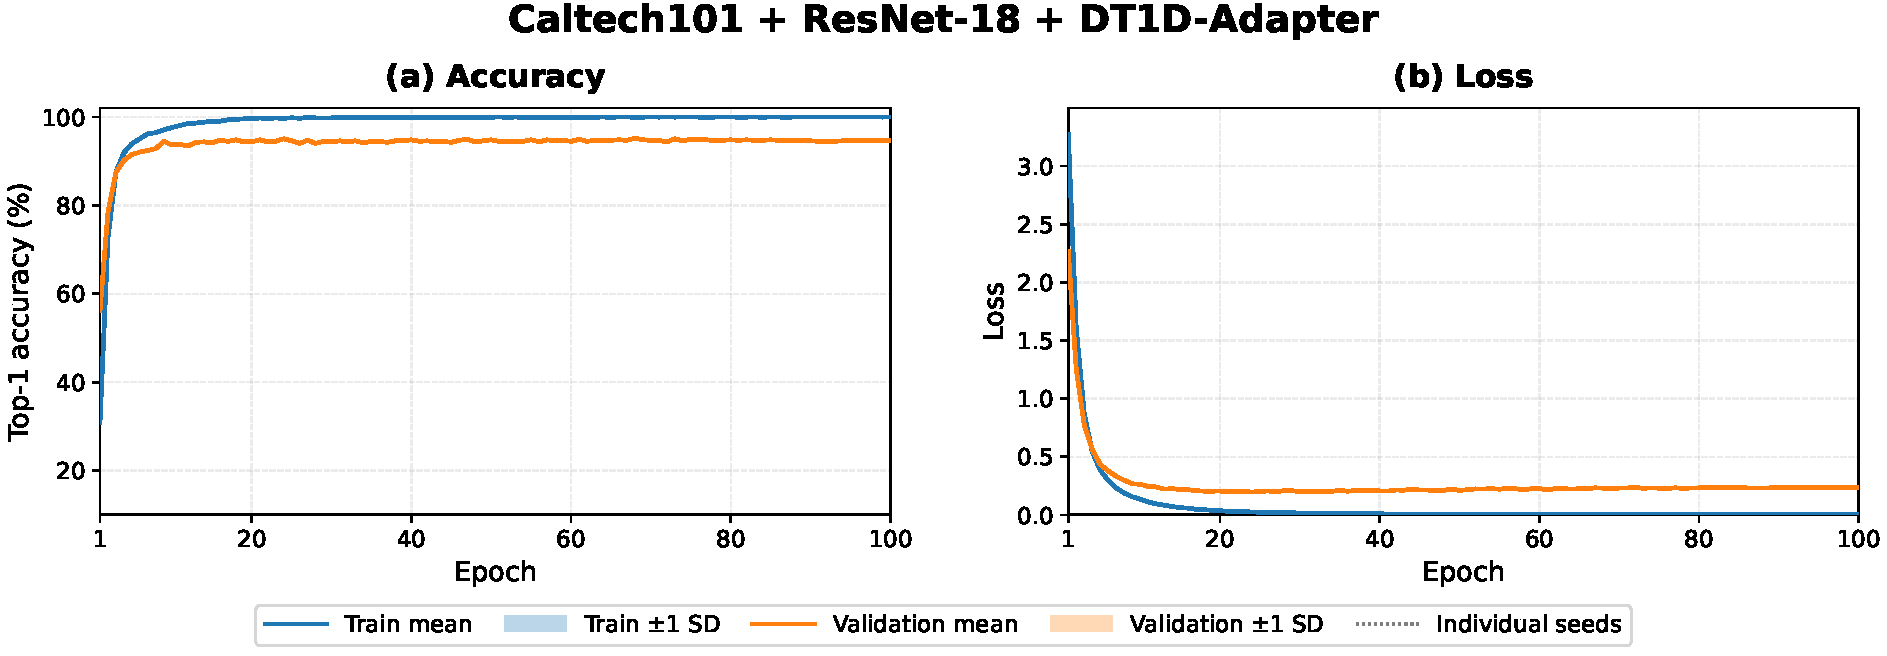
\includegraphics[width=0.94\textwidth]{figure_01.pdf}
\caption{Convergence behavior of DT1D-Adapter on Caltech101~\cite{fei2007caltech101} with an ImageNet-pretrained ResNet-18 backbone for the current F01 seed-0 rerun. The learning rate is selected by validation-only search over $\{10^{-4},3\times10^{-4},10^{-3},3\times10^{-3},5\times10^{-3}\}$; the selected learning rate is $3\times10^{-4}$. The best validation Acc@1 is $95.161\%$ at recorded epoch 67, and the corresponding one-time test evaluation gives $93.541\%$ Acc@1.}
\label{fig:caltech101_resnet18_dt1d_behavior}
\end{figure*}

Figure~\ref{fig:caltech101_resnet18_dt1d_behavior} shows the current F01 convergence trace for the selected validation-only configuration.


\section{Related Work}
\label{sec:Relatedwork}
Parameter-efficient fine-tuning (PEFT) in vision can be broadly grouped into prompt tuning, adapter-based tuning, low-rank or partial-parameter tuning, feature modulation, and convolutional or residual adaptation branches. 
This section reviews these directions with emphasis on their mechanisms, strengths, and limitations, and positions \textbf{DT1D-Adapter} relative to convolutional, residual, and axis-aware lightweight adaptation methods.

Prompt tuning learns task-specific tokens while keeping the pretrained backbone frozen. 
Visual Prompt Tuning (VPT)~\cite{jia2022vpt} is a representative approach for Vision Transformers and is attractive because it introduces only a small number of trainable parameters. 
Neural prompt search methods such as NOAH~\cite{zhang2025noah} further study automated prompt and adaptation design for Transformer-based vision models. 
However, prompt tuning is naturally tied to token-based representations and is less direct for convolutional feature maps, where spatial information is represented as dense $H\times W$ tensors. 
This motivates adapter designs that can operate directly on spatial feature maps and are not restricted to Transformer token sequences.

Adapter-based tuning inserts small trainable modules into a frozen backbone. 
Classical adapters were introduced as compact bottleneck modules~\cite{houlsby2019adapter}, and vision-oriented variants such as AdaptFormer~\cite{chen2022adaptformer}, FacT~\cite{jie2023fact}, Lv-Adapter~\cite{xu2024lvadapter}, CLIP-Adapter~\cite{gao2024clipadapter}, and meta-regularized PEFT~\cite{park2026peftmetar} study different lightweight adaptation mechanisms for Transformer or vision-language backbones. 
These methods demonstrate the effectiveness of adding compact trainable components to pretrained models, but many of them are primarily designed around Transformer block structures. 
By contrast, DT1D-Adapter is formulated on spatial feature tensors and can therefore be inserted into both ConvNet and ViT backbones after reshaping token features into spatial maps.

Vision-specific adapters introduce stronger spatial inductive bias. 
ConvPass~\cite{jie2024convpass} adds convolutional components to ViT adaptation, while RepAdapter~\cite{luo2023repadapter} uses structural re-parameterization to reduce inference-time overhead. 
ViT-Adapter~\cite{chen2023vitadapter} further shows that adapter-style spatial priors can help Transformer backbones serve dense vision tasks, and structured pruning adapters~\cite{hedegaard2024spa} provide another route for reducing adaptation cost. 
These works support the importance of spatial structure in visual adaptation. 
However, convolution-based branches may still introduce non-negligible parameter or computational cost depending on the kernel size, channel mixing, and insertion strategy. 
DT1D-Adapter follows this spatial-adaptation direction but restricts the learned spatial operator to group-shared symmetric axial base kernels with a low-dimensional channel-dependent correction, thereby avoiding a fully parameterized two-dimensional adaptation branch.

Low-rank and partial-parameter methods provide another lightweight PEFT route. 
LoRA~\cite{hu2022lora} learns low-rank weight updates, and later variants such as LoRand~\cite{yin2023lorand} further explore low-rank randomized adaptation. 
Recent visual low-rank adaptation studies, such as HLoRA-MER~\cite{shao2025hlora}, further show that high-level LoRA-style adaptation can be effective for visual recognition while maintaining a small trainable-parameter budget. 
BitFit~\cite{zaken2022bitfit} updates only bias parameters, SSF~\cite{lian2022ssf} learns feature-wise scale and shift parameters, and MoNA~\cite{yin2025mona} represents a recent vision-oriented PEFT direction. 
These methods are simple and storage-efficient, but they mainly modify parameter subspaces or feature statistics rather than explicitly modeling local or directional spatial structure. 
Therefore, they are complementary to DT1D-Adapter, which introduces a restricted structured axial filtering branch while keeping the backbone frozen.

Conv-Adapter~\cite{chen2024convadapter} and Residual Adapters~\cite{rebuffi2017residual} are among the closest baselines to our work. 
Conv-Adapter introduces convolutional adaptation modules for ConvNet backbones, while Residual Adapters use residual branches to adapt a shared backbone across domains. 
Both lines demonstrate the usefulness of residual adaptation with visual inductive bias. 
However, their parameter cost can grow with the branch design, the number of inserted layers, and the amount of channel mixing. 
DT1D-Adapter follows the residual-adaptation principle but constrains the spatial branch through a group-shared symmetric base response, a low-dimensional channel-dependent correction, a learned bounded symmetric coefficient shift fused into each axial kernel, post-shift joint height--width normalization, and a scalar residual gate.

Attention-style and axis-aware lightweight modules are also relevant. 
Squeeze-and-Excitation Networks~\cite{hu2020senet} and BAM~\cite{park2020lightweightattention} show that lightweight channel or channel--spatial recalibration can improve convolutional representations. 
Axial Attention~\cite{ho2019axialattention} and Axial-DeepLab~\cite{wang2020axialdeeplab} show that processing visual representations along separate spatial axes can reduce the cost of multidimensional modeling, while Coordinate Attention~\cite{hou2021coordinateattention} encodes direction-aware spatial information through separated height and width contexts. 
Large-kernel and depthwise-convolutional designs such as ConvNeXt~\cite{liu2022convnext} and RepLKNet~\cite{ding2022replknet} also support the usefulness of efficient spatial filtering in modern vision backbones. Efficient multi-scale processing is further explored by EAPT, which introduces an attention-pyramid Transformer for image-processing tasks~\cite{lin2023eapt}. Although EAPT is a complete visual architecture rather than a PEFT module, its design provides relevant context for efficient Transformer-based spatial representation learning. 
Taken together, these studies motivate axis-aware and depthwise spatial operations, while DT1D-Adapter specializes these principles to parameter-efficient fine-tuning through a compact structured axial-filtering branch.

Recent studies on efficient visual adaptation and lightweight model design further indicate the importance of reducing adaptation cost while preserving transfer performance. Examples include parameter-diminish fine-tuning for Transformer-based models~\cite{zhang2025pdft}, lightweight CNN--ViT designs~\cite{zhang2025lightweightcnnvit}, and environment-aware domain adaptation~\cite{zhu2024ceal}. 
For dense medical-image prediction, Wen et al.\ combine depthwise separable convolution with frequency-domain enhancement in a lightweight retinal-vessel segmentation network~\cite{wen2025retinalvessel}. Their design illustrates how compact spatial operators can support dense prediction while limiting model complexity. DT1D-Adapter addresses a complementary setting, namely the parameter-efficient adaptation of pretrained backbones, but shares the broader objective of introducing effective spatial modeling with a controlled task-specific parameter budget. A frozen-backbone RGB--IR detection framework with multi-receptive-field attention~\cite{lu2026frozenrgbir} provides another related example by combining fixed pretrained representations with lightweight task-specific adaptation and multi-scale receptive-field modeling. 
Collectively, these studies reinforce the broader trend toward efficient adaptation, compact spatial modeling, and reduced task-specific deployment cost.

Within this landscape, the individual operations used by DT1D-Adapter---axial filtering, depthwise convolution, symmetric kernels, shift operators, residual adaptation, and coefficient normalization---are established techniques. The distinction lies in how they are composed into a restricted task-specific spatial kernel family. Rather than learning an independent axial kernel for every channel, DT1D-Adapter shares a symmetric base kernel within each channel group, introduces only a low-dimensional channel-dependent correction, and learns a bounded axis-specific symmetric coefficient shift that is fused into the final axial kernel. This differs from axial attention and Coordinate Attention~\cite{ho2019axialattention,hou2021coordinateattention}, which construct content-dependent attention or directional context, whereas DT1D-Adapter remains a convolutional operator after training. The final formulation uses one finite-support kernel per enabled axis rather than evaluating several separate dilated-convolution branches~\cite{yu2016dilated}, and no input-dependent branch selection is used as in selective-kernel mechanisms~\cite{li2019sknet}. Compared with more general convolutional adapters, the proposed branch therefore restricts the learned spatial kernel family instead of introducing a freely parameterized two-dimensional spatial or channel-mixing module. Post-shift joint control of the height- and width-axis kernel magnitudes and gated residual injection complete the same compact spatial adaptation interface for ConvNet feature maps and spatially arranged ViT patch representations.

Table~\ref{tab:method_positioning} summarizes the position of DT1D-Adapter relative to representative PEFT and lightweight visual adaptation methods.


\begin{table*}[!t]
\centering
\caption{Positioning of DT1D-Adapter relative to representative PEFT and lightweight visual adaptation methods.}
\label{tab:method_positioning}
\small
\setlength{\tabcolsep}{5pt}
\renewcommand{\arraystretch}{1.18}
\begin{tabularx}{\textwidth}{|P{0.17\textwidth}|L|L|L|}
\hline
\textbf{Method family} &
\textbf{Main mechanism} &
\textbf{Main strength} &
\textbf{Relation to DT1D-Adapter} \\
\hline

VPT~\cite{jia2022vpt} &
Learnable prompt tokens for ViTs &
Very small trainable-parameter budget &
Token-based design; less direct for ConvNet feature maps. \\
\hline

AdaptFormer~\cite{chen2022adaptformer} &
Bottleneck adapter inside Transformer blocks &
Effective ViT adaptation &
Mainly designed for Transformer block structures. \\
\hline

LoRA~\cite{hu2022lora} &
Low-rank weight updates &
General and parameter-efficient &
Adapts weights but does not explicitly model spatial filtering. \\
\hline

BitFit / SSF~\cite{zaken2022bitfit,lian2022ssf} &
Bias tuning or feature-wise scale--shift tuning &
Extremely lightweight &
Modulates parameters or features without an explicit axial spatial prior. \\
\hline

ConvPass / Conv-Adapter~\cite{jie2024convpass,chen2024convadapter} &
Convolutional adaptation branch &
Strong visual inductive bias &
Spatially expressive, but parameter cost can increase with branch design. \\
\hline

Residual Adapters~\cite{rebuffi2017residual} &
Residual task- or domain-specific branches &
Effective multi-domain adaptation &
Related residual principle, but branch complexity may increase storage cost. \\
\hline

BAM-Tuning~\cite{park2020lightweightattention} &
Channel--spatial attention branch &
Lightweight feature recalibration &
Attention-based rather than structured axial-filtering based. \\
\hline

\textbf{DT1D-Adapter} &
Group-shared symmetric axial base and channel correction with fused bounded weighted shift &
Restricted spatial kernel family with controlled task-specific parameter cost &
One finite-support axial kernel per enabled axis; spatial PEFT interface for ConvNet maps and reshaped ViT patch grids. \\
\hline

\end{tabularx}
\end{table*}
The effectiveness of PEFT depends not only on the adaptation module, but also on its insertion location and parameter budget. 
This is important in vision backbones because early, middle, and deep layers represent different levels of texture, parts, and semantics. 
Therefore, PEFT methods should be evaluated with respect to accuracy, placement sensitivity, parameter budget, and backbone type.

SPT~\cite{he2023spt} studies sensitivity-based criteria for selecting task-relevant tuning locations and allocating parameters under a fixed budget. 
V-PETL~\cite{yu2022vpetl} further shows that placement and design choices can strongly affect transfer performance. 
Large-scale empirical studies also suggest that hyperparameter settings, training protocol, and parameter-budget alignment can change the ranking of PEFT methods~\cite{mai2025unifying}. 
These findings motivate our later discussion of insertion strategy and hyperparameter selection for DT1D-Adapter.

Fair evaluation is also important because PEFT methods differ in trainable parameters, storage cost, training memory, and inference overhead. 
Thus, accuracy alone can be misleading. 
V-PETL Bench~\cite{xin2024vpetlbench} provides a unified benchmark for vision PEFT, while recent surveys summarize evaluation settings and open challenges~\cite{yu2024visualtuning,xin2024visionpeftsurvey}. 
These studies motivate our experimental protocol, which reports accuracy, trainable parameters, storage cost, and computational or memory-related measurements where available.

\section{Mathematical Characterization and Design Rationale}
\label{sec:math_preliminaries}

This section characterizes the DT1D-Adapter parameterization used by the final implementation and relates its mathematical structure to the design choices used in the code. Standard finite-support convolution and Fourier analysis~\cite{grafakos2014classical,mallat2009wavelet} are used only as analytical tools to describe the restricted kernel family, the spectral effect of the learned weighted shift, and the post-shift joint kernel constraint.

\subsection{Structured shared and channel-dependent axial kernel}
\label{subsec:structured_kernel}

Let
\begin{equation}
x\in\mathbb{R}^{B\times C\times H\times W}
\end{equation}
be an intermediate feature tensor, and let
\begin{equation}
\mathcal{A}\subseteq\{h,w\}
\end{equation}
denote the enabled spatial axes. Channels are divided into groups of size $g_{\mathrm{ch}}$, with
\begin{equation}
G=\left\lceil \frac{C}{g_{\mathrm{ch}}}\right\rceil .
\end{equation}
For each axis $u\in\mathcal{A}$ and channel group $q$, DT1D-Adapter learns a symmetric group-shared base kernel over the fixed radii
\begin{equation}
\mathcal{R}=\{1,2,4\}.
\end{equation}
Writing $\delta_r$ for the unit impulse at offset $r$, the base component is
\begin{equation}
b_{u,q}
=
\beta_{u,q,0}\delta_0
+
\sum_{r\in\mathcal{R}}
\beta_{u,q,r}\left(\delta_{-r}+\delta_r\right).
\label{eq:dt1d_shared_base}
\end{equation}
Thus, the shared base response uses four learned coefficients per axis and group and occupies a direct 9-tap support from $-4$ to $+4$.

To allow limited channel-specific variation without learning an independent spatial kernel for every channel, DT1D-Adapter adds one channel-dependent correction component. Define the normalized symmetric second-difference basis function at radius 4
\begin{equation}
\psi_4
=
\frac{\delta_{-4}-2\delta_0+\delta_4}{\sqrt{6}},
\qquad
\sum_r \psi_4[r]=0,
\qquad
\|\psi_4\|_2=1.
\label{eq:dt1d_radius4_basis}
\end{equation}
Within every non-degenerate group, a fixed zero-mean within-group modulation vector $a_q$ is constructed so that
\begin{equation}
\mathbf{1}^{\top}a_q=0,
\qquad
\|a_q\|_2=1.
\label{eq:dt1d_channel_modulation}
\end{equation}
If channel $c$ belongs to group $g(c)$, its direct pre-shift axial kernel is
\begin{equation}
k_{u,c}
=
b_{u,g(c)}
+
\eta_{u,g(c)}\,a_c\,\psi_4,
\label{eq:dt1d_kernel}
\end{equation}
where $\eta_{u,g(c)}$ is a learned group-level correction amplitude. For a singleton remainder group, the zero-mean modulation is inactive, so the kernel reduces to the shared base component.

\subsection{Parameter efficiency and separation of shared and channel-dependent components}
\label{subsec:parameter_separation}

The structured parameterization reduces the learned spatial degrees of freedom at the group level.

\begin{proposition}[Spatial degrees of freedom]
\label{prop:dt1d_dof}
Consider a group containing $n\geq2$ channels. An unrestricted 13-tap depthwise axial filter has $13n$ free spatial coefficients for that group and axis. A per-channel symmetric kernel restricted to the coordinates $\{0,\pm1,\pm2,\pm4\}$ has $4n$ free coefficients. By contrast, the direct DT1D kernel family in \eqref{eq:dt1d_kernel} uses four group-shared base coefficients and one group-level correction amplitude, hence five learned spatial coefficients per group and axis before the weighted-shift scalar is applied.
\end{proposition}

\begin{proof}
The base kernel in \eqref{eq:dt1d_shared_base} belongs to the four-dimensional span
\[
\operatorname{span}\!\left\{
\delta_0,\,
\delta_{-1}+\delta_1,\,
\delta_{-2}+\delta_2,\,
\delta_{-4}+\delta_4
\right\}.
\]
The correction term adds one learned scalar coefficient $\eta_{u,q}$ along the fixed channel--spatial direction $a_q\psi_4^{\top}$. Since $a_q$ is nonzero and centered, this direction is linearly independent of the group-common base-kernel directions. Therefore the learned direct group-level spatial parameterization has five degrees of freedom.
\end{proof}

With $A=|\mathcal{A}|$ enabled axes, the direct shared/detail coefficients contribute
\begin{equation}
N_{\mathrm{direct}}=5AG,
\qquad
G=\left\lceil\frac{C}{g_{\mathrm{ch}}}\right\rceil,
\label{eq:dt1d_parameter_count}
\end{equation}
followed by $A$ learned axis-specific weighted-shift scalars and one learned residual gate in the canonical configuration. The reduction arises from restricting the channel--spatial kernel family rather than from merely replacing one convolution by another.

The same construction separates the common group response from the channel-dependent correction. For one group and axis, write the direct kernel tensor as
\begin{equation}
K_{u,q}
=
\mathbf{1}\,b_{u,q}^{\top}
+
\eta_{u,q}\,a_q\psi_4^{\top}.
\end{equation}

\begin{proposition}[Pre-shift orthogonality of shared and channel-dependent components]
\label{prop:dt1d_orthogonality}
The group-common base component and the channel-dependent correction component are orthogonal in the channel--spatial Frobenius inner product:
\begin{equation}
\left\langle
\mathbf{1}b_{u,q}^{\top},
\eta_{u,q}a_q\psi_4^{\top}
\right\rangle_F
=0.
\end{equation}
\end{proposition}

\begin{proof}
Using the separable form of the two terms and \eqref{eq:dt1d_channel_modulation},
\[
\left\langle
\mathbf{1}b^{\top},
\eta a\psi_4^{\top}
\right\rangle_F
=
\eta(\mathbf{1}^{\top}a)(b^{\top}\psi_4)
=0.
\]
\end{proof}

This orthogonality is a property of the direct shared/detail decomposition before the learned weighted shift and before the final per-channel projection. Practically, the shared component models the group-common spatial response, while the channel-dependent correction introduces limited channel variation without allocating a free kernel to every channel.

\subsection{Spectral structure, weighted shift, joint normalization, and residual control}
\label{subsec:spectral_stability}

Because the direct base kernel is symmetric, its one-dimensional Fourier response is real and even:
\begin{equation}
\widehat{b}_{u,q}(\omega)
=
\beta_{u,q,0}
+
2\sum_{r\in\{1,2,4\}}
\beta_{u,q,r}\cos(r\omega).
\label{eq:dt1d_shared_base_spectrum}
\end{equation}
The radius-4 correction basis function has response
\begin{equation}
\widehat{\psi}_4(\omega)
=
\frac{2\cos(4\omega)-2}{\sqrt{6}}
=
-\frac{4}{\sqrt{6}}\sin^2(2\omega),
\label{eq:dt1d_correction_spectrum}
\end{equation}
and therefore $\widehat{\psi}_4(0)=0$.

The final proposal then applies a learned symmetric coefficient shift to each enabled axis. For displacement $p=2$, let $S_{\pm2}$ denote a two-sample shift of a finite kernel on the expanded support and define
\begin{equation}
\bar{k}_{u,c}
=
\mathcal{W}_{2,\lambda_u}k_{u,c}
=
(1-\lambda_u)k_{u,c}
+
\frac{\lambda_u}{2}\left(S_{-2}k_{u,c}+S_{+2}k_{u,c}\right),
\label{eq:dt1d_weighted_shift}
\end{equation}
where
\begin{equation}
\lambda_u=0.5\tanh(\theta_u).
\label{eq:dt1d_shift_lambda}
\end{equation}
The height and width axes use independent learned scalars. They are initialized at $\lambda_u=0$, so training starts from the direct kernel in \eqref{eq:dt1d_kernel}. The direct radius is four and the shift displacement is two, giving an effective radius of six and an effective 13-tap kernel. The shift is fused into the kernel coefficients and therefore does not create an additional convolution branch.

For a finite kernel $k$ with Fourier response $\widehat{k}(\omega)$, the weighted shift has response
\begin{equation}
\widehat{\mathcal{W}_{2,\lambda}k}(\omega)
=
\left[1-\lambda+\lambda\cos(2\omega)\right]\widehat{k}(\omega).
\label{eq:dt1d_weighted_shift_spectrum}
\end{equation}
Thus, the learned scalar gives a bounded axis-specific spectral reweighting of the structured kernel rather than a content-dependent routing mechanism. Figure~\ref{fig:dt1d_structure} illustrates the compact direct spectral response and the $p=2$ weighted-shift multiplier. The plotted nonzero $\lambda$ is illustrative; the learned shift is initialized at zero in the actual model.

After the weighted shift, the implementation jointly projects the height and width kernels for each channel. Define
\begin{equation}
\rho_c
=
\max\!\left\{
1,\,
\|\bar{k}_{h,c}\|_1+\|\bar{k}_{w,c}\|_1
\right\},
\end{equation}
with the absent axis omitted in a single-axis configuration, and set
\begin{equation}
\widetilde{k}_{u,c}
=
\frac{\bar{k}_{u,c}}{\rho_c}.
\label{eq:dt1d_joint_projection}
\end{equation}
Then
\begin{equation}
\|\widetilde{k}_{h,c}\|_1+
\|\widetilde{k}_{w,c}\|_1
\leq1.
\label{eq:dt1d_joint_bound}
\end{equation}

\begin{proposition}[Bounded axial response under translation-invariant or zero-extension convolution]
\label{prop:dt1d_bounded}
Let
\begin{equation}
\mathcal{T}(x)_c
=
\widetilde{k}_{h,c}*_h x_c
+
\widetilde{k}_{w,c}*_w x_c.
\end{equation}
Under translation-invariant convolution or zero extension, for every $1\leq p\leq\infty$,
\begin{equation}
\|\mathcal{T}(x)\|_{\ell_p}
\leq
\|x\|_{\ell_p}.
\label{eq:dt1d_operator_bound}
\end{equation}
\end{proposition}

\begin{proof}
Young's convolution inequality gives
\[
\|\widetilde{k}_{h,c}*_h x_c\|_{\ell_p}
\leq
\|\widetilde{k}_{h,c}\|_1\|x_c\|_{\ell_p}
\]
and the analogous bound for the width axis. Combining the two estimates with \eqref{eq:dt1d_joint_bound} gives the result channel-wise and hence for the complete tensor.
\end{proof}

The implementation uses replicate padding as its finite-grid boundary treatment. We therefore use Proposition~\ref{prop:dt1d_bounded} to motivate the coefficient-mass projection itself and do not claim a general $\ell_p$ contraction for replicate padding. The corresponding pointwise/$\ell_\infty$ coefficient-mass control remains immediate from \eqref{eq:dt1d_joint_bound}.

Finally, the adapter output is
\begin{equation}
\operatorname{DT1D}(x)
=
x+s\gamma\,\mathcal{T}(x),
\label{eq:dt1d_residual}
\end{equation}
where $s=1$ and $\gamma$ is a learned scalar gate initialized at $0.01$. Under the same convolution assumptions,
\begin{equation}
\|\operatorname{DT1D}(x)-x\|_{\ell_p}
\leq
|s\gamma|\,\|x\|_{\ell_p}.
\end{equation}
Thus, the branch starts as a small near-identity perturbation, while the learned shift and gate respectively control the shape and magnitude of the structured spatial correction.

\begin{figure*}[!t]
\centering
\figureplaceholder{Spectral response figure: compact base response and weighted-shift multiplier.}
\caption{Spectral interpretation of the DT1D-Adapter parameterization. Placeholder reserved for the compact symmetric base response and the $p=2$ weighted-shift spectral modulation.}
\label{fig:dt1d_structure}
\end{figure*}

\section{Proposed Method}
\label{sec:proposed_method}

This section describes how the structured kernel from Section~\ref{sec:math_preliminaries} is used as a trainable residual branch in frozen visual backbones.

\subsection{Adapter architecture, axial filtering, and backbone insertion}
\label{subsec:axial_architecture}

Given a spatial feature map
\begin{equation}
x\in\mathbb{R}^{B\times C\times H\times W},
\end{equation}
DT1D-Adapter partitions the channels into groups of size $g_{\mathrm{ch}}=16$ and constructs the direct shared/detail kernel in \eqref{eq:dt1d_kernel} for each enabled spatial axis. It then applies the learned axis-specific weighted shift in \eqref{eq:dt1d_weighted_shift} and the post-shift joint $\ell_1$ projection in \eqref{eq:dt1d_joint_projection}. For related discrete weighted-convolution constructions, see Definition~1 (Eq.~(13)) of Huong and Ty~\cite{HuongTy2026Applications}, which defines a generalized $h$-Hartley--cosine convolution with weight $\gamma(y)=\cos(yh)$ on $\mathbb{T}_h$ and is subsequently interpreted as a discrete filtering mechanism. The two-axis response is
\begin{equation}
z
=
\operatorname{DWConv}_{13\times1}(x;\widetilde{k}_h)
+
\operatorname{DWConv}_{1\times13}(x;\widetilde{k}_w),
\label{eq:dt1d_axial_response}
\end{equation}
and the final output is
\begin{equation}
\mathrm{out}=x+s\gamma z,
\label{eq:dt1d_method_output}
\end{equation}
with residual scale $s=1$ and a learned gate initialized at $\gamma_0=0.01$. The branch requires one axial depthwise convolution per enabled axis; the weighted shift is already fused into the corresponding 13-tap kernel. A pointwise channel-mixing block is not used in the canonical proposal.

Because DT1D-Adapter operates on spatial tensors, it can be inserted into both CNN and Transformer backbones. For CNNs, intermediate activations already have shape $B\times C\times H\times W$, so the adapter can be inserted after selected convolutional blocks or residual stages, in the same general setting as lightweight residual visual adaptation~\cite{rebuffi2017residual,li2024repadapter}. During fine-tuning, the backbone remains frozen while the DT1D parameters, the two axis-specific shift scalars, the residual gate, and the task-specific head are updated.

For Vision Transformers~\cite{dosovitskiy2021vit}, the patch-token sequence is reshaped to a two-dimensional grid. If $N=H_pW_p$ patch tokens have embedding dimension $C$, the patch features are represented as
\begin{equation}
x\in\mathbb{R}^{B\times C\times H_p\times W_p},
\end{equation}
adapted with the same DT1D operator, and then reshaped back to the token sequence. A class token, when present, is kept separate and concatenated back after the patch tokens are restored. This gives the method a common spatial adaptation interface across ConvNet maps and ViT patch grids.

\begin{figure*}[!t]
\centering
\figureplaceholder{DT1D-Adapter architecture diagram.}
\caption{Architecture of the final DT1D-Adapter data path. Placeholder reserved for compact shared/detail kernel formation, the fused $p=2$ weighted shift, post-shift joint height--width projection, two axial depthwise convolutions, fusion, and learned residual injection.}
\label{fig:dt1d_architecture}
\end{figure*}

Figure~\ref{fig:dt1d_architecture} summarizes the complete data path of the final proposal: compact shared/detail kernel formation, the fused $p=2$ weighted shift, post-shift joint height--width projection, two axial depthwise convolutions, fusion, and learned residual injection.


\subsection{Configuration, computational cost, and algorithm}
\label{subsec:dt1d_cost}

Unless otherwise stated, DT1D-Adapter uses both spatial axes, channel-group size $g_{\mathrm{ch}}=16$, direct symmetric radii $\{1,2,4\}$, the normalized radius-4 second-difference basis function, learned axis-specific weighted shifts with $p=2$ and $\lambda_u=0.5\tanh\theta_u$ initialized at zero, joint $\ell_1$ projection applied after the weighted shift, a learned residual gate initialized at $0.01$, replicate padding, and no pointwise channel-mixing block. The direct kernel length is 9 and the effective shifted kernel length is $K=13$.

Ignoring the small cost of constructing and fusing the structured kernel coefficients, one depthwise axial convolution costs approximately
\begin{equation}
\mathcal{O}(BCHWK).
\end{equation}
With $A=|\mathcal{A}|$ enabled axes, the filtering cost is therefore
\begin{equation}
\mathcal{O}(BCHWAK).
\label{eq:dt1d_cost}
\end{equation}
For the two-axis configuration with $K=13$, the axial factor is $2K=26$, compared with $K^2=169$ for a full $13\times13$ depthwise spatial kernel over the same effective support. This comparison describes arithmetic structure only; it does not imply universally lower wall-clock latency, which also depends on tensor shapes, memory traffic, backend implementation, adapter placement, and hardware kernel efficiency.

\begin{algorithm}[h]
\caption{DT1D-Adapter on a feature tensor}
\label{alg:dt1d}
\begin{algorithmic}[1]
\Require Feature tensor $x$; group size $g_{\mathrm{ch}}=16$; shared-base coefficients $\beta$; correction amplitudes $\eta$; shift parameters $\theta_h,\theta_w$; residual gate $\gamma$
\Ensure $\mathrm{out}$ with the same shape as $x$
\State Partition the $C$ channels into $G=\lceil C/g_{\mathrm{ch}}\rceil$ groups
\For{each enabled axis $u\in\mathcal{A}$}
 \For{each channel group $q$}
  \State Construct the symmetric base kernel $b_{u,q}$ on $\{0,\pm1,\pm2,\pm4\}$
  \State Form the centered channel-dependent correction $\eta_{u,q}a_q\psi_4$
  \State Assign the direct kernel $k_{u,c}\gets b_{u,q}+\eta_{u,q}a_c\psi_4$ to each channel $c$ in group $q$
 \EndFor
 \State $\lambda_u\gets0.5\tanh(\theta_u)$
 \State Fuse the $p=2$ weighted shift $\bar{k}_{u,c}\gets(1-\lambda_u)k_{u,c}+\frac{\lambda_u}{2}(S_{-2}k_{u,c}+S_{+2}k_{u,c})$
\EndFor
\State Jointly project the shifted height and width kernels using \eqref{eq:dt1d_joint_projection}
\State $z_h\gets\operatorname{DWConv}_{13\times1}(x;\widetilde{k}_h)$
\State $z_w\gets\operatorname{DWConv}_{1\times13}(x;\widetilde{k}_w)$
\State $z\gets z_h+z_w$
\State $\mathrm{out}\gets x+\gamma z$
\State \Return $\mathrm{out}$
\end{algorithmic}
\end{algorithm}

\FloatBarrier



\section{Experiments}
\label{sec:impl-exp}

This section reports the results currently available from the supplied rerun archives. To avoid mixing current reruns with legacy values, only cells supported by the present result set are populated. All other numerical cells are intentionally left blank for later update. Likewise, result figures whose current outputs are not included in the supplied result set are retained as labeled placeholders.

\subsection{Experimental protocol}
\label{subsec:experimental_protocol}

The current result set includes the previously incorporated completed or partially completed reruns together with the newly supplied C10, C11, and C13 CNN result archives and the updated D06/D07 dense-prediction archive. F01 provides a single-seed Caltech101/ResNet-18 100-epoch convergence rerun for DT1D-Adapter; F04 provides a single-seed FGVC-Aircraft/ResNet-18 10-epoch accuracy--parameter trade-off with seven currently completed methods; and C12 provides three-seed Caltech101/ResNet-18 10-epoch comparison results for seven currently completed methods. In F04 and C12, the missing current runs remain unreported rather than being filled from legacy results. First, the core CNN ablation uses DTD/ResNet-18 and Flowers102/ResNet-50 with seeds $\{0,1,2\}$. Second, the CNN comparison reruns for DTD/ResNet-50 and Flowers102/ResNet-50 use validation-only learning-rate selection over the common grid $\{10^{-4},3\times10^{-4},10^{-3},3\times10^{-3},5\times10^{-3}\}$, followed by test evaluation at the selected best-validation checkpoint. The available CNN comparison archives are partial, so only completed method rows are populated. Third, the supplied ViT-B/16 result sets use a validation-only method-specific learning-rate search on tuning seed 42 followed by final evaluation with seeds $\{0,1,2\}$. VTAB-DTD and VTAB-EuroSAT use the VTAB-1k \texttt{train800}/\texttt{val200}/official-test protocol, while Flowers102 uses its official train/validation/test split. Fourth, the completed D05 binary-mask segmentation rerun evaluates nine methods on PennFudan using DeepLabV3-MobileNetV3-Large with input size $224\times224$, batch size 8, 100 epochs, AdamW, learning rate $10^{-3}$, weight decay $10^{-4}$, and seeds $\{0,1,2\}$. For each segmentation seed, the best checkpoint is selected by validation IoU and the test split is evaluated once. Fifth, the completed D04A/D04B PennFudan ViT-B/16 dense-decoder rerun evaluates DT1D-Adapter, Linear probing, BitFit, and Full fine-tuning with input size $224\times224$, batch size 8, 100 epochs, AdamW, learning rate $10^{-3}$, weight decay $10^{-4}$, cosine learning-rate scheduling, and seeds $\{0,1,2\}$. The best checkpoint for each seed is selected by validation IoU, with the test split evaluated once at that checkpoint. Sixth, the updated D06 object-detection rerun evaluates DT1D-Adapter, Full fine-tuning, the task-head-only baseline, Conv-Adapter, and BAM on Oxford-IIIT Pet detection with Faster R-CNN/MobileNetV3-FPN for 10 epochs using input size $320\times320$, batch size 1, AdamW with learning rate $10^{-3}$ and weight decay $10^{-4}$, cosine learning-rate scheduling, GPU execution, and seeds $\{0,1,2\}$. For every seed, the checkpoint with the highest validation detection metric is selected and the test split is evaluated once. Seventh, the completed D07 semantic-segmentation rerun evaluates DT1D-Adapter, Linear probing, BitFit, and Full fine-tuning on Oxford-IIIT Pet with a ViT-B/16 dense decoder for 5 epochs using input size $224\times224$, batch size 8, AdamW with learning rate $10^{-3}$ and weight decay $10^{-4}$, cosine learning-rate scheduling, and seeds $\{0,1,2\}$. The best checkpoint for each seed is selected by validation mIoU and the test split is evaluated once. Eighth, C10 provides a complete three-seed Oxford-IIIT Pet/EfficientNet-B0 10-epoch comparison with validation-only method-level learning-rate selection, while C11 targets the corresponding 100-epoch setting but currently contains complete final results only for Linear probing and BitFit. Ninth, C13 targets EuroSAT/MobileNetV3-Small for 25 epochs with batch size 32 and the same validation-only method-level learning-rate-selection rule; the supplied C13 archive currently contains complete final results only for Linear probing. Tenth, the completed D03 semantic-segmentation rerun evaluates DT1D-Adapter, Full fine-tuning, Linear probing, Conv-Adapter ($r=4$), and BAM on Oxford-IIIT Pet using DeepLabV3-MobileNetV3 for 5 epochs with input size $224\times224$, batch size 8, learning rate $10^{-3}$, weight decay $10^{-4}$, and seeds $\{0,1,2\}$. For each seed, the best checkpoint is selected by validation mIoU and the test split is evaluated once at that checkpoint.

For classification, top-1 accuracy is the primary metric. Where available, we also report top-5 accuracy, test loss, trainable parameters, parameter ratio, FP32 task storage, FLOPs, latency, throughput, training time, and memory use. For binary segmentation, we report foreground-class IoU and Dice together with global pixel accuracy, trainable parameters, task-specific FP32 storage, latency, training memory, and epoch time. For semantic segmentation, we report macro-class mIoU and Dice together with global pixel accuracy, parameter counts, task-specific FP32 storage, latency, throughput, inference and training memory, epoch time, and total training time. For object detection, we report $\mathrm{AP}_{50}$, $\mathrm{Recall}_{50}$, ground-truth and prediction counts, parameter counts, task-specific storage, latency, throughput, memory, epoch time, and total training time. Blank entries do not represent zero values; they indicate that the corresponding current rerun result has not yet been supplied.

\subsection{Experimental results}
\label{subsec:experimental_results}

\subsubsection{Ablation and hyperparameter sensitivity}
\label{subsec:ablation_sensitivity}

We evaluate four configurations to isolate the contributions of the structured kernel parameterization, the learned weighted shift, and the post-shift joint $\ell_1$ projection: DT1D-Adapter, the structured core without the weighted shift, the structured core without the joint $\ell_1$ projection, and an unrestricted axial depthwise 1D control.

\begin{table*}[!t]
\centering
\caption{Core ablation of DT1D-Adapter on DTD/ResNet-18 and Flowers102/ResNet-50. Results are reported as mean $\pm$ sample standard deviation over seeds $\{0,1,2\}$. Test Acc@1 is evaluated at the best-validation checkpoint, and latency is reported per image.}
\label{tab:dt1d_component_ablation}
\small
\setlength{\tabcolsep}{4.0pt}
\renewcommand{\arraystretch}{1.12}
\resizebox{\textwidth}{!}{%
\begin{tabular}{lrrrrrr}
\toprule
\multirow{2}{*}{\textbf{Configuration}} &
\multicolumn{3}{c}{\textbf{DTD / ResNet-18}} &
\multicolumn{3}{c}{\textbf{Flowers102 / ResNet-50}}\\
\cmidrule(lr){2-4}\cmidrule(lr){5-7}
& \makecell{\textbf{Trainable}\\\textbf{params}}
& \makecell{\textbf{Test Acc@1}\\\textbf{(\%)}}
& \makecell{\textbf{Latency}\\\textbf{(ms/img)}}
& \makecell{\textbf{Trainable}\\\textbf{params}}
& \makecell{\textbf{Test Acc@1}\\\textbf{(\%)}}
& \makecell{\textbf{Latency}\\\textbf{(ms/img)}}\\
\midrule
\textbf{DT1D-Adapter} & 25,335 & $62.163\pm0.406$ & $1.758\pm0.131$ & 218,486 & $81.477\pm0.551$ & $6.177\pm0.092$ \\
Without weighted shift & 25,319 & $61.986\pm0.201$ & $1.602\pm0.041$ & 218,454 & $81.417\pm0.628$ & $5.687\pm0.038$ \\
Without joint $\ell_1$ projection & 25,335 & $61.613\pm0.354$ & $1.074\pm0.006$ & 218,486 & $79.910\pm0.316$ & $6.114\pm0.043$ \\
Unrestricted axial depthwise 1D & 89,399 & $61.418\pm0.374$ & $1.152\pm0.004$ & 722,550 & $80.577\pm0.277$ & $6.591\pm0.074$ \\
\bottomrule
\end{tabular}%
}
\end{table*}

The ablation results show that the weighted shift provides a modest accuracy increment over the no-shift structured core: $+0.177$ percentage point on DTD and $+0.060$ point on Flowers102. Removing the post-shift joint $\ell_1$ projection produces a larger decrease, from $62.163\%$ to $61.613\%$ on DTD and from $81.477\%$ to $79.910\%$ on Flowers102. Relative to the unrestricted axial depthwise control, DT1D-Adapter reduces trainable parameters from 89,399 to 25,335 on DTD and from 722,550 to 218,486 on Flowers102 while slightly increasing mean test Acc@1 in both settings. These results support a parameter-compact structured operating point; they do not establish universal wall-clock superiority.

\FloatBarrier
\subsubsection{CNN-backbone image classification}

The current DTD/ResNet-50 and Flowers102/ResNet-50 reruns are only partially complete. Tables~\ref{tab:dtd_r50_100_3seed} and~\ref{tab:flowers102_r50_100} therefore populate only completed method rows from the supplied current result archives and retain the remaining rows as blanks.

\begin{table*}[!t]
\centering
\caption{Current three-seed comparison on DTD with an ImageNet-pretrained ResNet-50 backbone trained for 100 epochs using batch size 128. Values are populated only for completed rows in the supplied current result set; all other cells are intentionally left blank.}
\label{tab:dtd_r50_100_3seed}
\scriptsize
\setlength{\tabcolsep}{2.6pt}
\renewcommand{\arraystretch}{1.08}

\textbf{(a) Predictive performance and parameter/storage efficiency}
\vspace{2pt}
\resizebox{\textwidth}{!}{%
\begin{tabular}{@{}lrrrrrrrr@{}}
\toprule
\textbf{Method} &
\makecell{\textbf{Trainable}\\\textbf{params}} &
\makecell{\textbf{Total}\\\textbf{params}} &
\makecell{\textbf{Trainable}\\\textbf{(\%)}} &
\makecell{\textbf{FP32 storage/task}\\\textbf{(MiB)}} &
\makecell{\textbf{Best val}\\\textbf{Acc@1 (\%)}} &
\makecell{\textbf{Test Acc@1}\\\textbf{(\%)}} &
\makecell{\textbf{Test Acc@5}\\\textbf{(\%)}} &
\makecell{\textbf{Test}\\\textbf{loss}} \\
\midrule
\textbf{DT1D-Adapter} &  &  &  &  &  &  &  &  \\
Full fine-tuning &  &  &  &  &  &  &  &  \\
Linear probing & 96,303 & 23,604,335 & 0.408 & 0.367 & $71.028\pm0.081$ & $70.691\pm0.349$ & $92.748\pm0.163$ & $1.120\pm0.049$ \\
BitFit~\cite{zaken2022bitfit} & 122,863 & 23,604,335 & 0.521 & 0.469 & $71.418\pm0.494$ & $72.163\pm0.342$ & $92.695\pm0.630$ & $1.403\pm0.097$ \\
SSF~\cite{lian2022ssf} &  &  &  &  &  &  &  &  \\
Conv-Adapter~\cite{chen2024convadapter} ($r=2$) &  &  &  &  &  &  &  &  \\
Conv-Adapter~\cite{chen2024convadapter} ($r=4$) &  &  &  &  &  &  &  &  \\
Conv-Adapter~\cite{chen2024convadapter} ($r=6$) & 6,810,724 & 30,318,756 & 22.464 & 25.981 & $70.390\pm0.111$ & $71.294\pm0.111$ & $92.411\pm0.342$ & $1.689\pm0.317$ \\
Conv-Adapter~\cite{chen2024convadapter} ($r=8$) & 5,143,183 & 28,651,215 & 17.951 & 19.620 & $70.177\pm0.494$ & $71.011\pm0.435$ & $92.376\pm0.187$ & $1.666\pm0.040$ \\
Residual Adapters~\cite{rebuffi2017residual} &  &  &  &  &  &  &  &  \\
\bottomrule
\end{tabular}%
}

\vspace{5pt}
\textbf{(b) Computational and runtime efficiency}
\vspace{2pt}
\resizebox{\textwidth}{!}{%
\begin{tabular}{@{}lrrrrrr@{}}
\toprule
\textbf{Method} &
\makecell{\textbf{FLOPs}\\\textbf{(G)}} &
\makecell{\textbf{Latency}\\\textbf{(ms/img)}} &
\textbf{FPS} &
\makecell{\textbf{Training time}\\\textbf{(s)}} &
\makecell{\textbf{Peak train}\\\textbf{memory (MB)}} &
\makecell{\textbf{Peak inference}\\\textbf{memory (MB)}} \\
\midrule
\textbf{DT1D-Adapter} &  &  &  &  &  &  \\
Full fine-tuning &  &  &  &  &  &  \\
Linear probing & 4.110 & $1.425\pm0.010$ & $701.609\pm4.904$ & $2393.565\pm15.112$ & 868.530 & 194.592 \\
BitFit~\cite{zaken2022bitfit} & 4.110 & $1.473\pm0.027$ & $678.937\pm12.684$ & $2470.389\pm5.889$ & 5603.667 & 194.592 \\
SSF~\cite{lian2022ssf} &  &  &  &  &  &  \\
Conv-Adapter~\cite{chen2024convadapter} ($r=2$) &  &  &  &  &  &  \\
Conv-Adapter~\cite{chen2024convadapter} ($r=4$) &  &  &  &  &  &  \\
Conv-Adapter~\cite{chen2024convadapter} ($r=6$) & 5.208 & $2.165\pm0.022$ & $462.017\pm4.653$ & $2622.093\pm36.883$ & 6275.117 & 238.792 \\
Conv-Adapter~\cite{chen2024convadapter} ($r=8$) & 4.938 & $1.962\pm0.035$ & $509.854\pm9.001$ & $2608.979\pm30.208$ & 6149.434 & 235.568 \\
Residual Adapters~\cite{rebuffi2017residual} &  &  &  &  &  &  \\
\bottomrule
\end{tabular}%
}
\vspace{2pt}
{\footnotesize\textit{Blank cells indicate method results not yet available in the current result set.}}
\end{table*}

\begin{table*}[!t]
\centering
\caption{Current three-seed comparison on Flowers102 with an ImageNet-pretrained ResNet-50 backbone trained for 100 epochs using batch size 128. Values are populated only for completed rows in the supplied current result set; all other cells are intentionally left blank.}
\label{tab:flowers102_r50_100}
\scriptsize
\setlength{\tabcolsep}{2.6pt}
\renewcommand{\arraystretch}{1.08}

\textbf{(a) Predictive performance and parameter/storage efficiency}
\vspace{2pt}
\resizebox{\textwidth}{!}{%
\begin{tabular}{@{}lrrrrrrrr@{}}
\toprule
\textbf{Method} &
\makecell{\textbf{Trainable}\\\textbf{params}} &
\makecell{\textbf{Total}\\\textbf{params}} &
\makecell{\textbf{Trainable}\\\textbf{(\%)}} &
\makecell{\textbf{FP32 storage/task}\\\textbf{(MiB)}} &
\makecell{\textbf{Best val}\\\textbf{Acc@1 (\%)}} &
\makecell{\textbf{Test Acc@1}\\\textbf{(\%)}} &
\makecell{\textbf{Test Acc@5}\\\textbf{(\%)}} &
\makecell{\textbf{Test}\\\textbf{loss}} \\
\midrule
\textbf{DT1D-Adapter} &  &  &  &  &  &  &  &  \\
Full fine-tuning &  &  &  &  &  &  &  &  \\
Linear probing & 208,998 & 23,717,030 & 0.881 & 0.797 & $84.118\pm0.170$ & $82.431\pm0.123$ & $94.102\pm0.146$ & $0.756\pm0.011$ \\
BitFit~\cite{zaken2022bitfit} & 235,558 & 23,717,030 & 0.993 & 0.899 & $85.882\pm0.784$ & $84.903\pm0.593$ & $95.972\pm0.122$ & $0.606\pm0.010$ \\
SSF~\cite{lian2022ssf} &  &  &  &  &  &  &  &  \\
Conv-Adapter~\cite{chen2024convadapter} ($r=2$) &  &  &  &  &  &  &  &  \\
Conv-Adapter~\cite{chen2024convadapter} ($r=4$) &  &  &  &  &  &  &  &  \\
Conv-Adapter~\cite{chen2024convadapter} ($r=6$) &  &  &  &  &  &  &  &  \\
Conv-Adapter~\cite{chen2024convadapter} ($r=8$) &  &  &  &  &  &  &  &  \\
Residual Adapters~\cite{rebuffi2017residual} &  &  &  &  &  &  &  &  \\
\bottomrule
\end{tabular}%
}

\vspace{5pt}
\textbf{(b) Computational and runtime efficiency}
\vspace{2pt}
\resizebox{\textwidth}{!}{%
\begin{tabular}{@{}lrrrrrr@{}}
\toprule
\textbf{Method} &
\makecell{\textbf{FLOPs}\\\textbf{(G)}} &
\makecell{\textbf{Latency}\\\textbf{(ms/img)}} &
\textbf{FPS} &
\makecell{\textbf{Training time}\\\textbf{(s)}} &
\makecell{\textbf{Peak train}\\\textbf{memory (MB)}} &
\makecell{\textbf{Peak inference}\\\textbf{memory (MB)}} \\
\midrule
\textbf{DT1D-Adapter} &  &  &  &  &  &  \\
Full fine-tuning &  &  &  &  &  &  \\
Linear probing & 4.110 & $1.391\pm0.006$ & $719.067\pm3.063$ & $1513.376\pm20.313$ & 869.833 & 195.022 \\
BitFit~\cite{zaken2022bitfit} & 4.110 & $1.420\pm0.003$ & $704.100\pm1.349$ & $1545.136\pm15.266$ & 5605.399 & 195.022 \\
SSF~\cite{lian2022ssf} &  &  &  &  &  &  \\
Conv-Adapter~\cite{chen2024convadapter} ($r=2$) &  &  &  &  &  &  \\
Conv-Adapter~\cite{chen2024convadapter} ($r=4$) &  &  &  &  &  &  \\
Conv-Adapter~\cite{chen2024convadapter} ($r=6$) &  &  &  &  &  &  \\
Conv-Adapter~\cite{chen2024convadapter} ($r=8$) &  &  &  &  &  &  \\
Residual Adapters~\cite{rebuffi2017residual} &  &  &  &  &  &  \\
\bottomrule
\end{tabular}%
}
\vspace{2pt}
{\footnotesize\textit{Blank cells indicate method results not yet available in the current result set.}}
\end{table*}

The supplied C03 archive completes the Flowers102/ResNet-18 10-epoch, batch-size-64 comparison in Table~\ref{tab:flowers102_r18_10}. It contains successful three-seed runs for DT1D-Adapter, Full fine-tuning, Linear probing, BitFit, SSF, and Conv-Adapter with bottleneck ratios $r\in\{2,4,6,8\}$ under the same validation-only learning-rate selection protocol. Methods not present in C03 remain blank rather than carrying forward legacy values.

\begin{table*}[!t]
\centering
\caption{Three-seed accuracy, parameter/storage, and runtime comparison on Flowers102 with an ImageNet-pretrained ResNet-18 backbone trained for 10 epochs using batch size 64. Results are reported over independent seeds $\{0,1,2\}$. For each seed, the test set is evaluated at the checkpoint with the highest validation $\mathrm{Acc}_{1}$. Runtime profiling uses $224\times224$ inputs with profile batch size 16 on an NVIDIA Tesla T4.}
\label{tab:flowers102_r18_10}
\scriptsize
\setlength{\tabcolsep}{3.2pt}
\renewcommand{\arraystretch}{1.08}

\textbf{(a) Predictive performance and parameter/storage efficiency}

\vspace{2pt}
\resizebox{\textwidth}{!}{%
\begin{tabular}{@{}lrrrrrr@{}}
\toprule
\textbf{Method} &
\makecell{\textbf{Trainable}\\\textbf{params}} &
\makecell{\textbf{Total params}\\\textbf{(M)}} &
\makecell{\textbf{Trainable}\\\textbf{(\%)}} &
\makecell{\textbf{FP32 storage/task}\\\textbf{(MB)}} &
\makecell{\textbf{Best val}\\\textbf{$\mathrm{Acc}_{1}$ (\%)}} &
\makecell{\textbf{Test $\mathrm{Acc}_{1}$}\\\textbf{at best val (\%)}} \\
\midrule
\textbf{DT1D-Adapter} & 53,550 & 11.230 & 0.477 & 0.214 & $84.542\pm0.786$ & $83.011\pm0.244$ \\
Full fine-tuning & 11,228,838 & 11.229 & 100.000 & 44.915 & $91.765\pm0.259$ & $88.415\pm0.206$ \\
Linear probing & 52,326 & 11.229 & 0.466 & 0.209 & $81.961\pm0.294$ & $80.490\pm0.461$ \\
BitFit~\cite{zaken2022bitfit} & 57,126 & 11.229 & 0.509 & 0.229 & $85.294\pm0.995$ & $83.157\pm0.474$ \\
SSF~\cite{lian2022ssf} & 56,166 & 11.233 & 0.500 & 0.225 & $83.922\pm0.980$ & $83.103\pm0.818$ \\
BAM~\cite{park2020lightweightattention} &  &  &  &  &  & \\
Residual Adapters~\cite{rebuffi2017residual} &  &  &  &  &  & \\
LoRA-Conv~\cite{hu2022lora} &  &  &  &  &  & \\
Side-Tuning~\cite{zhang2020sidetuning} &  &  &  &  &  & \\
Conv-Adapter~\cite{chen2024convadapter} ($r=8$) & 228,566 & 11.405 & 2.004 & 0.914 & $84.118\pm1.968$ & $81.899\pm0.685$ \\
Conv-Adapter~\cite{chen2024convadapter} ($r=6$) & 285,570 & 11.462 & 2.491 & 1.142 & $82.614\pm2.206$ & $80.322\pm1.690$ \\
Conv-Adapter~\cite{chen2024convadapter} ($r=4$) & 404,806 & 11.581 & 3.495 & 1.619 & $81.961\pm1.444$ & $79.970\pm0.939$ \\
Conv-Adapter~\cite{chen2024convadapter} ($r=2$) & 757,286 & 11.934 & 6.346 & 3.029 & $82.320\pm1.374$ & $80.485\pm0.918$ \\
\bottomrule
\end{tabular}%
}

\vspace{5pt}
\textbf{(b) Computational, runtime, and memory efficiency}

\vspace{2pt}
\resizebox{\textwidth}{!}{%
\begin{tabular}{@{}lrrrrrr@{}}
\toprule
\textbf{Method} &
\makecell{\textbf{FLOPs}\\\textbf{(G)}} &
\makecell{\textbf{Latency}\\\textbf{(ms/img)}} &
\textbf{FPS} &
\makecell{\textbf{Peak train}\\\textbf{memory (MB)}} &
\makecell{\textbf{Peak inference}\\\textbf{memory (MB)}} &
\makecell{\textbf{Train time}\\\textbf{(s)}} \\
\midrule
\textbf{DT1D-Adapter} & 3.686 & $1.770\pm0.117$ & $566.421\pm36.216$ & 897.613 & 127.926 & $138.071\pm0.138$ \\
Full fine-tuning & 1.819 & $0.546\pm0.007$ & $1831.536\pm24.530$ & 959.242 & 120.960 & $88.878\pm1.116$ \\
Linear probing & 1.819 & $0.548\pm0.007$ & $1825.648\pm23.080$ & 336.219 & 120.960 & $131.959\pm1.159$ \\
BitFit~\cite{zaken2022bitfit} & 1.819 & $0.545\pm0.002$ & $1834.391\pm6.970$ & 851.074 & 120.960 & $132.978\pm0.562$ \\
SSF~\cite{lian2022ssf} & 1.819 & $0.599\pm0.008$ & $1668.718\pm23.610$ & 600.114 & 120.976 & $132.597\pm0.275$ \\
BAM~\cite{park2020lightweightattention} &  &  &  &  &  & \\
Residual Adapters~\cite{rebuffi2017residual} &  &  &  &  &  & \\
LoRA-Conv~\cite{hu2022lora} &  &  &  &  &  & \\
Side-Tuning~\cite{zhang2020sidetuning} &  &  &  &  &  & \\
Conv-Adapter~\cite{chen2024convadapter} ($r=8$) & 1.845 & $0.627\pm0.002$ & $1593.857\pm4.622$ & 570.274 & 121.635 & $132.149\pm2.149$ \\
Conv-Adapter~\cite{chen2024convadapter} ($r=6$) & 1.853 & $0.625\pm0.002$ & $1599.951\pm4.988$ & 578.688 & 121.851 & $136.481\pm2.630$ \\
Conv-Adapter~\cite{chen2024convadapter} ($r=4$) & 1.872 & $0.633\pm0.005$ & $1579.792\pm12.870$ & 595.580 & 122.307 & $135.171\pm1.453$ \\
Conv-Adapter~\cite{chen2024convadapter} ($r=2$) & 1.925 & $0.640\pm0.015$ & $1563.334\pm37.210$ & 644.254 & 123.650 & $140.239\pm1.238$ \\
\bottomrule
\end{tabular}%
}

\vspace{2pt}
\parbox{\textwidth}{\scriptsize
FP32 storage/task is computed as four bytes per trainable task-specific parameter.
Latency, FPS, and training time are reported as mean $\pm$ sample standard deviation over the three seeds; parameter counts, FLOPs, and the reported peak-memory values are constant across the three runs for each method in this experiment.
The FLOP values follow the repository profiler. For DT1D-Adapter, the profiler explicitly adds the functional axial operations that are not represented as ordinary traced modules; these figures should therefore be interpreted as implementation-level compute estimates rather than exact hardware-independent operation counts.
}

\vspace{2pt}
{\footnotesize\textit{Blank cells indicate methods not included in the supplied C03 archive.}}
\end{table*}

The completed C03 comparison shows that Full fine-tuning obtains the highest mean test Acc@1 at $88.415\pm0.206\%$. Among the supplied parameter-efficient methods, BitFit ($83.157\pm0.474\%$), SSF ($83.103\pm0.818\%$), and DT1D-Adapter ($83.011\pm0.244\%$) form the strongest accuracy group. DT1D-Adapter uses 53,550 trainable parameters (0.477\% of the 11.230M-parameter model), close to Linear probing, BitFit, and SSF, but its functional axial operations raise the profiler estimate to 3.686~G FLOPs and $1.770\pm0.117$~ms/image latency. The C03 result therefore supports parameter compactness without implying a wall-clock advantage over the simpler PEFT baselines.


% v6: Result-table environments with zero verified numerical entries were removed.
% They should be reintroduced only after a complete verified rerun exists.


\begin{table*}[!htbp]
\centering
\caption{Three-seed accuracy, parameter, and storage results on Oxford-IIIT Pet with EfficientNet-B0 trained for 10 epochs using batch size 64. A single learning rate is selected for each method by mean best-validation Acc@1 across seeds $\{0,1,2\}$ from the common grid $\{10^{-4},3\times10^{-4},10^{-3},3\times10^{-3},5\times10^{-3}\}$, and each seed is evaluated once on the test set at its best-validation checkpoint. Values that vary across seeds are reported as mean $\pm$ sample standard deviation.}
\label{tab:pet_effb0_10}
\scriptsize
\setlength{\tabcolsep}{3.2pt}
\renewcommand{\arraystretch}{1.10}
\resizebox{\textwidth}{!}{%
\begin{tabular}{@{}lrrrrrrrr@{}}
\toprule
\textbf{Method} &
\makecell{\textbf{Trainable}\\\textbf{params}} &
\makecell{\textbf{Total}\\\textbf{params}} &
\makecell{\textbf{Trainable}\\\textbf{(\%)}} &
\makecell{\textbf{FP32 storage/task}\\\textbf{(MiB)}} &
\makecell{\textbf{Best val}\\\textbf{Acc@1 (\%)}} &
\makecell{\textbf{Test Acc@1}\\\textbf{(\%)}} &
\makecell{\textbf{Test Acc@5}\\\textbf{(\%)}} &
\makecell{\textbf{Test}\\\textbf{loss}} \\
\midrule
\textbf{DT1D-Adapter} & 48,595 & 4,056,143 & 1.198 & 0.185 & $92.618\pm1.699$ & $91.905\pm0.109$ & $99.700\pm0.072$ & $0.271\pm0.006$ \\
Full fine-tuning & 4,054,945 & 4,054,945 & 100.000 & 15.468 & $91.531\pm0.905$ & $89.552\pm0.659$ & $99.255\pm0.031$ & $0.340\pm0.016$ \\
Linear probing & 47,397 & 4,054,945 & 1.169 & 0.181 & $92.889\pm1.340$ & $91.878\pm0.191$ & $99.646\pm0.072$ & $0.255\pm0.004$ \\
Conv-Adapter~\cite{chen2024convadapter} ($r=4$) & 207,113 & 4,214,661 & 4.914 & 0.790 & $93.025\pm1.660$ & $91.987\pm0.179$ & $99.646\pm0.055$ & $0.280\pm0.009$ \\
Conv-Adapter~\cite{chen2024convadapter} ($r=2$) & 366,829 & 4,374,377 & 8.386 & 1.399 & $93.161\pm1.218$ & $91.651\pm0.437$ & $99.628\pm0.042$ & $0.282\pm0.014$ \\
Conv-Adapter~\cite{chen2024convadapter} ($r=6$) & 152,877 & 4,160,425 & 3.675 & 0.583 & $93.207\pm1.338$ & $91.769\pm0.428$ & $99.582\pm0.083$ & $0.285\pm0.005$ \\
Conv-Adapter~\cite{chen2024convadapter} ($r=8$) & 127,255 & 4,134,803 & 3.078 & 0.485 & $93.116\pm1.139$ & $91.823\pm0.361$ & $99.555\pm0.042$ & $0.280\pm0.013$ \\
SSF~\cite{lian2022ssf} & 51,013 & 4,058,561 & 1.257 & 0.195 & $92.889\pm1.225$ & $91.878\pm0.233$ & $99.618\pm0.119$ & $0.249\pm0.008$ \\
BitFit~\cite{zaken2022bitfit} & 77,745 & 4,054,945 & 1.917 & 0.297 & $93.207\pm1.184$ & $91.842\pm0.873$ & $99.582\pm0.063$ & $0.267\pm0.012$ \\
Prompt/VPT~\cite{jia2022vpt} &  &  &  &  &  &  &  & \\
\bottomrule
\end{tabular}%
}
\vspace{2pt}
{\footnotesize\textit{Blank cells indicate results not available in the supplied C10 archive. FP32 storage/task is computed from the trainable-parameter count using four bytes per parameter.}}
\end{table*}

\begin{table*}[!htbp]
\centering
\caption{Three-seed efficiency and runtime results for the C10 Oxford-IIIT Pet/EfficientNet-B0 10-epoch experiment. FLOPs and profiler inference memory are architecture-level quantities; latency, throughput, training time, and epoch time are reported as mean $\pm$ sample standard deviation over seeds $\{0,1,2\}$. Profiling uses $224\times224$ inputs and profile batch size 16.}
\label{tab:pet_effb0_10_efficiency}
\scriptsize
\setlength{\tabcolsep}{3.4pt}
\renewcommand{\arraystretch}{1.10}
\resizebox{\textwidth}{!}{%
\begin{tabular}{@{}lrrrrrrr@{}}
\toprule
\textbf{Method} &
\makecell{\textbf{FLOPs}\\\textbf{(G)}} &
\makecell{\textbf{Latency}\\\textbf{(ms/img)}} &
\textbf{FPS} &
\makecell{\textbf{Train time}\\\textbf{(s)}} &
\makecell{\textbf{Epoch time}\\\textbf{(s)}} &
\makecell{\textbf{Peak train}\\\textbf{memory (MB)}} &
\makecell{\textbf{Peak inference}\\\textbf{memory (MB)}} \\
\midrule
\textbf{DT1D-Adapter} & 0.858 & $3.995\pm0.466$ & $252.500\pm27.868$ & $254.893\pm2.535$ & $20.282\pm0.077$ & 2715.984 & 113.891 \\
Full fine-tuning & 0.400 & $0.748\pm0.001$ & $1337.496\pm2.443$ & $168.802\pm17.358$ & $13.373\pm1.355$ & 2847.094 & 113.651 \\
Linear probing & 0.400 & $0.895\pm0.209$ & $1153.934\pm239.490$ & $219.959\pm0.371$ & $17.092\pm0.124$ & 390.575 & 113.643 \\
Conv-Adapter~\cite{chen2024convadapter} ($r=4$) & 0.418 & $1.242\pm0.157$ & $814.260\pm111.021$ & $231.187\pm0.999$ & $18.052\pm0.218$ & 2537.708 & 114.264 \\
Conv-Adapter~\cite{chen2024convadapter} ($r=2$) & 0.436 & $1.375\pm0.222$ & $740.934\pm125.287$ & $233.791\pm12.732$ & $18.318\pm0.971$ & 2577.825 & 114.868 \\
Conv-Adapter~\cite{chen2024convadapter} ($r=6$) & 0.412 & $1.580\pm0.078$ & $634.087\pm30.575$ & $232.263\pm2.371$ & $18.125\pm0.261$ & 2527.269 & 114.056 \\
Conv-Adapter~\cite{chen2024convadapter} ($r=8$) & 0.409 & $1.386\pm0.260$ & $738.858\pm141.259$ & $230.261\pm2.460$ & $18.112\pm0.283$ & 2523.712 & 113.958 \\
SSF~\cite{lian2022ssf} & 0.400 & $1.024\pm0.171$ & $996.028\pm173.789$ & $243.797\pm3.266$ & $19.227\pm0.263$ & 2504.972 & 119.789 \\
BitFit~\cite{zaken2022bitfit} & 0.400 & $0.891\pm0.128$ & $1138.954\pm168.141$ & $227.078\pm2.338$ & $17.831\pm0.298$ & 2802.236 & 113.644 \\
Prompt/VPT~\cite{jia2022vpt} &  &  &  &  &  &  & \\
\bottomrule
\end{tabular}%
}
\vspace{2pt}
{\footnotesize\textit{Blank cells indicate results not available in the supplied C10 archive. Latency, FPS, FLOPs, and peak inference memory are taken from the released efficiency profiler; training-memory and timing values come from the completed training runs.}}
\end{table*}

\begin{table*}[!htbp]
\centering
\caption{Current three-seed accuracy, parameter, and storage results on Oxford-IIIT Pet with EfficientNet-B0 trained for 100 epochs using batch size 64. The supplied C11 archive is partial: only Linear probing and BitFit contain complete final results for seeds $\{0,1,2\}$. Values that vary across seeds are reported as mean $\pm$ sample standard deviation; incomplete method rows remain blank.}
\label{tab:pet_effb0_100}
\scriptsize
\setlength{\tabcolsep}{3.2pt}
\renewcommand{\arraystretch}{1.10}
\resizebox{\textwidth}{!}{%
\begin{tabular}{@{}lrrrrrrrr@{}}
\toprule
\textbf{Method} &
\makecell{\textbf{Trainable}\\\textbf{params}} &
\makecell{\textbf{Total}\\\textbf{params}} &
\makecell{\textbf{Trainable}\\\textbf{(\%)}} &
\makecell{\textbf{FP32 storage/task}\\\textbf{(MiB)}} &
\makecell{\textbf{Best val}\\\textbf{Acc@1 (\%)}} &
\makecell{\textbf{Test Acc@1}\\\textbf{(\%)}} &
\makecell{\textbf{Test Acc@5}\\\textbf{(\%)}} &
\makecell{\textbf{Test}\\\textbf{loss}} \\
\midrule
\textbf{DT1D-Adapter} &  &  &  &  &  &  &  & \\
Full fine-tuning &  &  &  &  &  &  &  & \\
Linear probing & 47,397 & 4,054,945 & 1.169 & 0.181 & $93.207\pm1.078$ & $91.678\pm0.265$ & $99.509\pm0.072$ & $0.281\pm0.021$ \\
Conv-Adapter~\cite{chen2024convadapter} ($r=4$) &  &  &  &  &  &  &  & \\
Conv-Adapter~\cite{chen2024convadapter} ($r=2$) &  &  &  &  &  &  &  & \\
Conv-Adapter~\cite{chen2024convadapter} ($r=6$) &  &  &  &  &  &  &  & \\
Conv-Adapter~\cite{chen2024convadapter} ($r=8$) &  &  &  &  &  &  &  & \\
SSF~\cite{lian2022ssf} &  &  &  &  &  &  &  & \\
BitFit~\cite{zaken2022bitfit} & 77,745 & 4,054,945 & 1.917 & 0.297 & $93.659\pm1.621$ & $91.251\pm0.330$ & $99.382\pm0.063$ & $0.377\pm0.033$ \\
Prompt/VPT~\cite{jia2022vpt} &  &  &  &  &  &  &  & \\
\bottomrule
\end{tabular}%
}
\vspace{2pt}
{\footnotesize\textit{Blank cells indicate method results not complete in the supplied C11 archive. FP32 storage/task is computed from the trainable-parameter count using four bytes per parameter.}}
\end{table*}

\begin{table*}[!htbp]
\centering
\caption{Current efficiency and runtime results for the C11 Oxford-IIIT Pet/EfficientNet-B0 100-epoch experiment. Only Linear probing and BitFit have complete three-seed final results in the supplied archive. Profiling uses $224\times224$ inputs and profile batch size 16.}
\label{tab:pet_effb0_100_efficiency}
\scriptsize
\setlength{\tabcolsep}{3.4pt}
\renewcommand{\arraystretch}{1.10}
\resizebox{\textwidth}{!}{%
\begin{tabular}{@{}lrrrrrrr@{}}
\toprule
\textbf{Method} &
\makecell{\textbf{FLOPs}\\\textbf{(G)}} &
\makecell{\textbf{Latency}\\\textbf{(ms/img)}} &
\textbf{FPS} &
\makecell{\textbf{Train time}\\\textbf{(s)}} &
\makecell{\textbf{Epoch time}\\\textbf{(s)}} &
\makecell{\textbf{Peak train}\\\textbf{memory (MB)}} &
\makecell{\textbf{Peak inference}\\\textbf{memory (MB)}} \\
\midrule
\textbf{DT1D-Adapter} &  &  &  &  &  &  & \\
Full fine-tuning &  &  &  &  &  &  & \\
Linear probing & 0.400 & $0.895\pm0.114$ & $1128.917\pm143.909$ & $2104.642\pm20.456$ & $16.615\pm0.204$ & 390.575 & 113.643 \\
Conv-Adapter~\cite{chen2024convadapter} ($r=4$) &  &  &  &  &  &  & \\
Conv-Adapter~\cite{chen2024convadapter} ($r=2$) &  &  &  &  &  &  & \\
Conv-Adapter~\cite{chen2024convadapter} ($r=6$) &  &  &  &  &  &  & \\
Conv-Adapter~\cite{chen2024convadapter} ($r=8$) &  &  &  &  &  &  & \\
SSF~\cite{lian2022ssf} &  &  &  &  &  &  & \\
BitFit~\cite{zaken2022bitfit} & 0.400 & $0.956\pm0.059$ & $1048.913\pm66.429$ & $2139.431\pm19.836$ & $17.017\pm0.234$ & 2802.236 & 113.644 \\
Prompt/VPT~\cite{jia2022vpt} &  &  &  &  &  &  & \\
\bottomrule
\end{tabular}%
}
\vspace{2pt}
{\footnotesize\textit{Blank cells indicate method results not complete in the supplied C11 archive. Latency, FPS, FLOPs, and peak inference memory are taken from the released efficiency profiler; training-memory and timing values come from the completed training runs.}}
\end{table*}

The completed C10 rerun shows a narrow accuracy spread among the PEFT baselines on Oxford-IIIT Pet/EfficientNet-B0 at 10 epochs. Conv-Adapter ($r=4$) records the highest supplied mean test Acc@1 at $91.987\pm0.179\%$, while DT1D-Adapter reaches $91.905\pm0.109\%$ with 48,595 trainable parameters, corresponding to 1.198\% of the 4.056M-parameter model and approximately 0.185~MiB of FP32 task-specific storage. Linear probing and SSF both reach $91.878\%$ mean test Acc@1, and the supplied Full fine-tuning run reaches $89.552\pm0.659\%$. The runtime profile makes the trade-off explicit: DT1D-Adapter requires 0.858~G FLOPs and $3.995\pm0.466$~ms/image ($252.500\pm27.868$ FPS), whereas Linear probing requires 0.400~G FLOPs and $0.895\pm0.209$~ms/image and Conv-Adapter ($r=4$) requires 0.418~G FLOPs and $1.242\pm0.157$~ms/image. Thus, the C10 result supports parameter/storage compactness but not a claim of lower inference latency. The C11 100-epoch archive is incomplete; among the two methods with complete three-seed final results, Linear probing reaches $91.678\pm0.265\%$ with $0.895\pm0.114$~ms/image latency, while BitFit reaches $91.251\pm0.330\%$ with $0.956\pm0.059$~ms/image latency. No conclusion is drawn for the missing C11 methods until their final runs are supplied.


\begin{table*}[!htbp]
\centering
\caption{Accuracy and parameter results on Caltech101 with a ResNet-18 backbone trained for 10 epochs using batch size 64. Results are mean $\pm$ sample standard deviation over seeds $\{0,1,2\}$; for each seed, the test set is evaluated at the checkpoint with the highest validation $\mathrm{Acc}_{1}$. Trainable and total parameter counts are fixed by the corresponding method configuration.}
\label{tab:caltech101_resnet18_10ep_accuracy}
\scriptsize
\setlength{\tabcolsep}{4pt}
\renewcommand{\arraystretch}{1.12}
\resizebox{\textwidth}{!}{%
\begin{tabular}{@{}lrrrrrrr@{}}
\toprule
\textbf{Method} &
\makecell{\textbf{Trainable}\\\textbf{params}} &
\makecell{\textbf{Total}\\\textbf{params}} &
\makecell{\textbf{Best val}\\\textbf{acc. (\%)}} &
\makecell{\textbf{Best}\\\textbf{epoch}} &
\makecell{\textbf{Test}\\\textbf{$\mathrm{Acc}_{1}$ (\%)}} &
\makecell{\textbf{Test}\\\textbf{$\mathrm{Acc}_{5}$ (\%)}} &
\makecell{\textbf{Test}\\\textbf{loss}} \\
\midrule
\textbf{DT1D-Adapter} & 53,037 & 11,229,549 & $94.854\pm0.580$ & $7.667\pm0.577$ & $94.387\pm0.569$ & $99.116\pm0.266$ & $0.228\pm0.006$ \\
Full fine-tuning &  &  &  &  &  &  & \\
Linear probing & 51,813 & 11,228,325 & $93.894\pm0.610$ & $6.000\pm1.732$ & $93.349\pm0.656$ & $98.962\pm0.115$ & $0.255\pm0.022$ \\
Conv-Adapter~\cite{chen2024convadapter} ($r=4$) & 404,293 & 11,580,805 & $94.585\pm0.115$ & $7.000\pm1.732$ & $94.771\pm1.072$ & $99.154\pm0.067$ & $0.229\pm0.021$ \\
BAM~\cite{park2020lightweightattention} & 129,397 & 11,306,149 & $94.547\pm0.544$ & $7.667\pm1.528$ & $94.617\pm0.371$ & $99.308\pm0.115$ & $0.196\pm0.018$ \\
Residual Adapters~\cite{rebuffi2017residual} & 138,861 & 11,315,613 & $94.163\pm0.333$ & $5.667\pm1.155$ & $94.233\pm1.112$ & $99.000\pm0.290$ & $0.249\pm0.058$ \\
SSF~\cite{lian2022ssf} & 55,653 & 11,232,165 & $94.278\pm0.655$ & $7.000\pm1.000$ & $94.002\pm1.006$ & $99.193\pm0.346$ & $0.238\pm0.043$ \\
LoRA-Conv~\cite{hu2022lora} &  &  &  &  &  &  & \\
BitFit~\cite{zaken2022bitfit} & 56,613 & 11,228,325 & $95.315\pm0.133$ & $7.333\pm1.528$ & $94.887\pm0.240$ & $99.116\pm0.290$ & $0.208\pm0.027$ \\
Side-Tuning~\cite{zhang2020sidetuning} &  &  &  &  &  &  & \\
\bottomrule
\end{tabular}%
}

\vspace{2pt}
{\footnotesize\textit{Blank cells indicate current C12 results not yet available for Full fine-tuning, LoRA-Conv, and Side-Tuning.}}
\end{table*}

\begin{table*}[!htbp]
\centering
\caption{Efficiency and runtime results on Caltech101 with a ResNet-18 backbone trained for 10 epochs using batch size 64. Latency, FPS, training time, and epoch time are reported as mean $\pm$ sample standard deviation over seeds $\{0,1,2\}$; FLOPs are architecture-level quantities and are unchanged across seeds.}
\label{tab:caltech101_resnet18_10ep_efficiency}
\scriptsize
\setlength{\tabcolsep}{5pt}
\renewcommand{\arraystretch}{1.12}
\resizebox{\textwidth}{!}{%
\begin{tabular}{@{}lrrrrr@{}}
\toprule
\textbf{Method} &
\makecell{\textbf{FLOPs}\\\textbf{(G)}} &
\makecell{\textbf{Latency}\\\textbf{(ms/img)}} &
\textbf{FPS} &
\makecell{\textbf{Train}\\\textbf{time (s)}} &
\makecell{\textbf{Epoch}\\\textbf{time (s)}} \\
\midrule
\textbf{DT1D-Adapter} & 3.686 & $2.066\pm0.407$ & $498.651\pm110.640$ & $368.394\pm1.492$ & $33.287\pm0.113$ \\
Full fine-tuning &  &  &  &  & \\
Linear probing & 1.819 & $0.504\pm0.003$ & $1983.352\pm13.669$ & $252.866\pm4.450$ & $22.020\pm0.357$ \\
Conv-Adapter~\cite{chen2024convadapter} ($r=4$) & 1.872 & $0.612\pm0.004$ & $1633.496\pm10.273$ & $174.410\pm0.911$ & $15.239\pm0.100$ \\
BAM~\cite{park2020lightweightattention} & 1.824 & $0.575\pm0.002$ & $1738.976\pm4.715$ & $272.247\pm3.909$ & $23.813\pm0.402$ \\
Residual Adapters~\cite{rebuffi2017residual} & 1.832 & $0.607\pm0.002$ & $1646.252\pm6.711$ & $169.362\pm1.249$ & $14.861\pm0.111$ \\
SSF~\cite{lian2022ssf} & 1.819 & $0.581\pm0.013$ & $1722.256\pm37.576$ & $287.861\pm22.735$ & $25.376\pm2.028$ \\
LoRA-Conv~\cite{hu2022lora} &  &  &  &  & \\
BitFit~\cite{zaken2022bitfit} & 1.819 & $0.498\pm0.003$ & $2006.915\pm11.521$ & $253.714\pm1.699$ & $22.312\pm0.175$ \\
Side-Tuning~\cite{zhang2020sidetuning} &  &  &  &  & \\
\bottomrule
\end{tabular}%
}

\vspace{2pt}
{\footnotesize\textit{Blank cells indicate current C12 results not yet available for Full fine-tuning, LoRA-Conv, and Side-Tuning.}}
\end{table*}

The current C12 results place the completed Caltech101/ResNet-18 methods in a narrow accuracy range. BitFit has the highest completed mean test Acc@1 at $94.887\pm0.240\%$, followed by Conv-Adapter at $94.771\pm1.072\%$, BAM at $94.617\pm0.371\%$, and DT1D-Adapter at $94.387\pm0.569\%$. DT1D-Adapter uses 53,037 trainable parameters, close to Linear probing, SSF, and BitFit; its C12 profile reports 3.686~G FLOPs and $2.066\pm0.407$~ms/image latency. Full fine-tuning, LoRA-Conv, and Side-Tuning remain blank because those current C12 runs are not present in the supplied archive.

\FloatBarrier

% -----------------------------------------------------------------------------
% v10 ADDITIONAL small-dataset CNN templates.
% Exactly four logical experiments, each assigned one backbone.
% -----------------------------------------------------------------------------
The additional CNN-only evaluation contains exactly four small-dataset experiments rather than a Cartesian product of datasets and backbones. N01 uses EfficientNet-B0 on STL10 for 10 epochs; N02 uses MobileNetV3-Small on Oxford Flowers17 for 10 epochs; N03 uses DenseNet-121~\cite{huang2017densenet} on STL10 for 100 epochs; and N04 uses ResNet-18 on Oxford Flowers17 for 100 epochs. This provides compound-scaled, mobile-oriented, densely connected, and residual backbone coverage while keeping the additional experimental scope compact. The same ten-method baseline family, seeds $\{0,1,2\}$, and validation-only shared-learning-rate rule are used in all four settings.

\begin{table*}[!htbp]
\centering
\caption{Reserved v10 result-entry template for N01: STL10~\cite{coates2011stl10} with EfficientNet-B0, trained for 10 epochs using batch size 64 and seeds $\{0,1,2\}$. The table is intentionally blank until each method has a complete three-seed aggregate after validation-only shared-learning-rate selection.}
\label{tab:additional_n01_stl10_efficientnet_b0_10ep}
\scriptsize
\setlength{\tabcolsep}{3.6pt}
\renewcommand{\arraystretch}{1.08}
\resizebox{\textwidth}{!}{%
\begin{tabular}{@{}lrrrrrr@{}}
\toprule
\textbf{Method} &
\makecell{\textbf{Trainable}\\\textbf{params}} &
\makecell{\textbf{Trainable}\\\textbf{(\%)}} &
\makecell{\textbf{Best val}\\\textbf{Acc@1 (\%)}} &
\makecell{\textbf{Test Acc@1}\\\textbf{(\%)}} &
\makecell{\textbf{FLOPs}\\\textbf{(G)}} &
\makecell{\textbf{Latency}\\\textbf{(ms/img)}} \\
\midrule
\textbf{DT1D-Adapter} & & & & & & \\
Full fine-tuning & & & & & & \\
Linear probing & & & & & & \\
BitFit~\cite{zaken2022bitfit} & & & & & & \\
SSF~\cite{lian2022ssf} & & & & & & \\
Conv-Adapter~\cite{chen2024convadapter} ($r=4$) & & & & & & \\
BAM~\cite{park2020lightweightattention} & & & & & & \\
Residual Adapters~\cite{rebuffi2017residual} & & & & & & \\
LoRA-Conv~\cite{hu2022lora} & & & & & & \\
Side-Tuning~\cite{zhang2020sidetuning} & & & & & & \\
\bottomrule
\end{tabular}%
}
\vspace{2pt}
{\footnotesize\textit{Blank cells are deliberate. Fill a method row only from the complete three-seed aggregate for this exact dataset/backbone/epoch setting; do not insert partial-session values.}}
\end{table*}

\begin{table*}[!htbp]
\centering
\caption{Reserved v10 result-entry template for N02: Oxford Flowers17~\cite{nilsback2006flowers17} with MobileNetV3-Small, trained for 10 epochs using batch size 64 and seeds $\{0,1,2\}$. The table is intentionally blank until each method has a complete three-seed aggregate after validation-only shared-learning-rate selection.}
\label{tab:additional_n02_flowers17_mobilenet_v3_small_10ep}
\scriptsize
\setlength{\tabcolsep}{3.6pt}
\renewcommand{\arraystretch}{1.08}
\resizebox{\textwidth}{!}{%
\begin{tabular}{@{}lrrrrrr@{}}
\toprule
\textbf{Method} &
\makecell{\textbf{Trainable}\\\textbf{params}} &
\makecell{\textbf{Trainable}\\\textbf{(\%)}} &
\makecell{\textbf{Best val}\\\textbf{Acc@1 (\%)}} &
\makecell{\textbf{Test Acc@1}\\\textbf{(\%)}} &
\makecell{\textbf{FLOPs}\\\textbf{(G)}} &
\makecell{\textbf{Latency}\\\textbf{(ms/img)}} \\
\midrule
\textbf{DT1D-Adapter} & & & & & & \\
Full fine-tuning & & & & & & \\
Linear probing & & & & & & \\
BitFit~\cite{zaken2022bitfit} & & & & & & \\
SSF~\cite{lian2022ssf} & & & & & & \\
Conv-Adapter~\cite{chen2024convadapter} ($r=4$) & & & & & & \\
BAM~\cite{park2020lightweightattention} & & & & & & \\
Residual Adapters~\cite{rebuffi2017residual} & & & & & & \\
LoRA-Conv~\cite{hu2022lora} & & & & & & \\
Side-Tuning~\cite{zhang2020sidetuning} & & & & & & \\
\bottomrule
\end{tabular}%
}
\vspace{2pt}
{\footnotesize\textit{Blank cells are deliberate. Fill a method row only from the complete three-seed aggregate for this exact dataset/backbone/epoch setting; do not insert partial-session values.}}
\end{table*}

\begin{table*}[!htbp]
\centering
\caption{Reserved v10 result-entry template for N03: STL10~\cite{coates2011stl10} with DenseNet-121~\cite{huang2017densenet}, trained for 100 epochs using batch size 64 and seeds $\{0,1,2\}$. The table is intentionally blank until each method has a complete three-seed aggregate after validation-only shared-learning-rate selection.}
\label{tab:additional_n03_stl10_densenet121_100ep}
\scriptsize
\setlength{\tabcolsep}{3.6pt}
\renewcommand{\arraystretch}{1.08}
\resizebox{\textwidth}{!}{%
\begin{tabular}{@{}lrrrrrr@{}}
\toprule
\textbf{Method} &
\makecell{\textbf{Trainable}\\\textbf{params}} &
\makecell{\textbf{Trainable}\\\textbf{(\%)}} &
\makecell{\textbf{Best val}\\\textbf{Acc@1 (\%)}} &
\makecell{\textbf{Test Acc@1}\\\textbf{(\%)}} &
\makecell{\textbf{FLOPs}\\\textbf{(G)}} &
\makecell{\textbf{Latency}\\\textbf{(ms/img)}} \\
\midrule
\textbf{DT1D-Adapter} & & & & & & \\
Full fine-tuning & & & & & & \\
Linear probing & & & & & & \\
BitFit~\cite{zaken2022bitfit} & & & & & & \\
SSF~\cite{lian2022ssf} & & & & & & \\
Conv-Adapter~\cite{chen2024convadapter} ($r=4$) & & & & & & \\
BAM~\cite{park2020lightweightattention} & & & & & & \\
Residual Adapters~\cite{rebuffi2017residual} & & & & & & \\
LoRA-Conv~\cite{hu2022lora} & & & & & & \\
Side-Tuning~\cite{zhang2020sidetuning} & & & & & & \\
\bottomrule
\end{tabular}%
}
\vspace{2pt}
{\footnotesize\textit{Blank cells are deliberate. Fill a method row only from the complete three-seed aggregate for this exact dataset/backbone/epoch setting; do not insert partial-session values.}}
\end{table*}

\begin{table*}[!htbp]
\centering
\caption{Reserved v10 result-entry template for N04: Oxford Flowers17~\cite{nilsback2006flowers17} with ResNet-18, trained for 100 epochs using batch size 64 and seeds $\{0,1,2\}$. The table is intentionally blank until each method has a complete three-seed aggregate after validation-only shared-learning-rate selection.}
\label{tab:additional_n04_flowers17_resnet18_100ep}
\scriptsize
\setlength{\tabcolsep}{3.6pt}
\renewcommand{\arraystretch}{1.08}
\resizebox{\textwidth}{!}{%
\begin{tabular}{@{}lrrrrrr@{}}
\toprule
\textbf{Method} &
\makecell{\textbf{Trainable}\\\textbf{params}} &
\makecell{\textbf{Trainable}\\\textbf{(\%)}} &
\makecell{\textbf{Best val}\\\textbf{Acc@1 (\%)}} &
\makecell{\textbf{Test Acc@1}\\\textbf{(\%)}} &
\makecell{\textbf{FLOPs}\\\textbf{(G)}} &
\makecell{\textbf{Latency}\\\textbf{(ms/img)}} \\
\midrule
\textbf{DT1D-Adapter} & & & & & & \\
Full fine-tuning & & & & & & \\
Linear probing & & & & & & \\
BitFit~\cite{zaken2022bitfit} & & & & & & \\
SSF~\cite{lian2022ssf} & & & & & & \\
Conv-Adapter~\cite{chen2024convadapter} ($r=4$) & & & & & & \\
BAM~\cite{park2020lightweightattention} & & & & & & \\
Residual Adapters~\cite{rebuffi2017residual} & & & & & & \\
LoRA-Conv~\cite{hu2022lora} & & & & & & \\
Side-Tuning~\cite{zhang2020sidetuning} & & & & & & \\
\bottomrule
\end{tabular}%
}
\vspace{2pt}
{\footnotesize\textit{Blank cells are deliberate. Fill a method row only from the complete three-seed aggregate for this exact dataset/backbone/epoch setting; do not insert partial-session values.}}
\end{table*}

\subsubsection{Transformer-backbone image classification}

The supplied current ViT result set contains complete three-seed results for Flowers102 at batch sizes 16 and 32 and for VTAB-Caltech101, VTAB-DTD, and VTAB-EuroSAT at batch size 32.

\begin{table*}[!t]
\centering
\caption{Three-seed ViT-B/16~\cite{dosovitskiy2021vit} results on Flowers102. Models are trained for 10 epochs at $224\times224$ resolution using seeds $\{0,1,2\}$. The supplied current result set contains complete batch-size-16 and batch-size-32 three-seed results.}
\label{tab:flowers102_vit_recovered_corrected}
\scriptsize
\setlength{\tabcolsep}{2.7pt}
\renewcommand{\arraystretch}{1.10}
\resizebox{\textwidth}{!}{%
\begin{tabular}{@{}rllrrrrrrrr@{}}
\toprule
\textbf{BS} & \textbf{Method} & \textbf{Opt. / LR} &
\makecell{\textbf{Trainable}\\\textbf{params}} &
\makecell{\textbf{Trainable}\\\textbf{(\%)}} &
\makecell{\textbf{FP32}\\\textbf{storage (MiB)}} &
\makecell{\textbf{Test Acc@1}\\\textbf{(\%)}} &
\makecell{\textbf{Test Acc@5}\\\textbf{(\%)}} &
\makecell{\textbf{Test}\\\textbf{loss}} &
\makecell{\textbf{Test batch}\\\textbf{time (s)}} &
\makecell{\textbf{Peak GPU}\\\textbf{mem. (GB)}} \\
\midrule
\multirow{5}{*}{32} & \textbf{DT1D-Adapter} & AdamW / $0.01$ & 84,234 & 0.098 & 0.321 & $96.092\pm0.203$ &  &  &  &  \\
 & Full fine-tuning & AdamW / $2.5\times10^{-4}$ & 85,877,094 & 100.000 & 327.595 & $95.858\pm0.156$ &  &  &  &  \\
 & Linear probing & SGD / $0.0625$ & 78,438 & 0.091 & 0.299 & $95.815\pm0.377$ &  &  &  &  \\
 & VPT~\cite{jia2022vpt} & SGD / $0.125$ & 82,278 & 0.096 & 0.314 & $95.858\pm0.272$ &  &  &  &  \\
 & Pfeiffer Adapter & AdamW / $2.5\times10^{-3}$ & 972,966 & 1.121 & 3.712 & $96.867\pm0.047$ &  &  &  &  \\
\midrule
\multirow{5}{*}{16} & \textbf{DT1D-Adapter} & AdamW / $0.01$ & 84,234 & 0.098 & 0.321 & $95.864\pm0.191$ &  &  &  &  \\
 & Full fine-tuning & AdamW / $3.125\times10^{-4}$ & 85,877,094 & 100.000 & 327.595 & $95.511\pm0.658$ &  &  &  &  \\
 & Linear probing & SGD / $0.03125$ & 78,438 & 0.091 & 0.299 & $95.533\pm0.292$ &  &  &  &  \\
 & VPT~\cite{jia2022vpt} & SGD / $0.625$ & 82,278 & 0.096 & 0.314 & $95.072\pm0.703$ &  &  &  &  \\
 & Pfeiffer Adapter & AdamW / $2.5\times10^{-3}$ & 972,966 & 1.121 & 3.712 & $96.471\pm0.181$ &  &  &  &  \\
\bottomrule
\end{tabular}%
}
\vspace{2pt}
{\footnotesize\textit{Blank ancillary cells indicate values not present in the supplied current result set.}}
\end{table*}

\begin{table*}[!t]
\centering
\caption{Three-seed comparison on VTAB-Caltech101 using ViT-B/16~\cite{dosovitskiy2021vit}. The VTAB-1k protocol uses \texttt{train800} for training, \texttt{val200} for validation, and the official test set for testing. All methods are trained for 10 epochs with batch size 32 and $224\times224$ inputs. Results are mean $\pm$ sample standard deviation over seeds $\{0,1,2\}$.}
\label{tab:vtab_caltech101_vit_recovered_corrected}
\scriptsize
\setlength{\tabcolsep}{4.0pt}
\renewcommand{\arraystretch}{1.10}
\resizebox{\textwidth}{!}{%
\begin{tabular}{@{}llrrrrr@{}}
\toprule
\textbf{Method} & \textbf{Opt. / LR} &
\makecell{\textbf{Trainable}\\\textbf{params}} &
\makecell{\textbf{Trainable}\\\textbf{(\%)}} &
\makecell{\textbf{FP32}\\\textbf{storage (MiB)}} &
\makecell{\textbf{Best val}\\\textbf{Acc@1 (\%)}} &
\makecell{\textbf{Test Acc@1}\\\textbf{(\%)}} \\
\midrule
\textbf{DT1D-Adapter} & AdamW / $0.01$ & 84,234 & 0.098 & 0.321 & $82.167\pm1.155$ & $82.249\pm1.078$ \\
Full fine-tuning & AdamW / $2.5\times10^{-4}$ & 85,877,094 & 100.000 & 327.595 & $82.667\pm1.607$ & $72.770\pm4.338$ \\
Linear probing & SGD / $0.0625$ & 78,438 & 0.091 & 0.299 & $82.833\pm2.021$ & $80.736\pm2.133$ \\
VPT~\cite{jia2022vpt} & SGD / $0.125$ & 86,118 & 0.100 & 0.329 & $83.000\pm1.803$ & $82.495\pm1.335$ \\
Pfeiffer Adapter & AdamW / $0.005$ & 972,966 & 1.121 & 3.712 & $82.000\pm2.784$ & $75.920\pm0.740$ \\
\bottomrule
\end{tabular}%
}
\end{table*}

\begin{table*}[!t]
\centering
\caption{Three-seed comparison on VTAB-DTD using ViT-B/16~\cite{dosovitskiy2021vit}. The VTAB-1k protocol uses \texttt{train800} for training, \texttt{val200} for validation, and the official test set for testing. All methods are trained for 10 epochs with batch size 32 and $224\times224$ inputs. Results are mean $\pm$ sample standard deviation over seeds $\{0,1,2\}$.}
\label{tab:vtab_dtd_vit_v01}
\scriptsize
\setlength{\tabcolsep}{4.0pt}
\renewcommand{\arraystretch}{1.10}
\resizebox{\textwidth}{!}{%
\begin{tabular}{@{}llrrrrr@{}}
\toprule
\textbf{Method} & \textbf{Opt. / LR} &
\makecell{\textbf{Trainable}\\\textbf{params}} &
\makecell{\textbf{Trainable}\\\textbf{(\%)}} &
\makecell{\textbf{FP32}\\\textbf{storage (MiB)}} &
\makecell{\textbf{Best val}\\\textbf{Acc@1 (\%)}} &
\makecell{\textbf{Test Acc@1}\\\textbf{(\%)}} \\
\midrule
\textbf{DT1D-Adapter} & AdamW / $0.01$ & 41,939 & 0.049 & 0.160 & $48.667\pm4.041$ & $49.450\pm1.413$ \\
Full fine-tuning & AdamW / $6.25\times10^{-4}$ & 85,834,799 & 100.000 & 327.434 & $52.833\pm0.764$ & $53.280\pm0.826$ \\
Linear probing & SGD / $6.25$ & 36,143 & 0.042 & 0.138 & $57.333\pm0.764$ & $55.106\pm0.555$ \\
VPT~\cite{jia2022vpt} & SGD / $1.25$ & 43,823 & 0.051 & 0.167 & $56.167\pm2.021$ & $55.142\pm1.518$ \\
Pfeiffer Adapter & AdamW / $0.01$ & 930,671 & 1.073 & 3.550 & $50.833\pm3.253$ & $51.223\pm1.778$ \\
\bottomrule
\end{tabular}%
}
\vspace{2pt}
{\footnotesize\textit{Blank cells indicate results not yet available in the current result set.}}
\end{table*}

\begin{table*}[!t]
\centering
\caption{Three-seed comparison on VTAB-EuroSAT using ViT-B/16~\cite{dosovitskiy2021vit}. The VTAB-1k protocol uses \texttt{train800} for training, \texttt{val200} for validation, and the official test set for testing. All methods are trained for 10 epochs with batch size 32 and $224\times224$ inputs. Results are mean $\pm$ sample standard deviation over seeds $\{0,1,2\}$.}
\label{tab:vtab_eurosat_vit_v02}
\scriptsize
\setlength{\tabcolsep}{4.0pt}
\renewcommand{\arraystretch}{1.10}
\resizebox{\textwidth}{!}{%
\begin{tabular}{@{}llrrrrr@{}}
\toprule
\textbf{Method} & \textbf{Opt. / LR} &
\makecell{\textbf{Trainable}\\\textbf{params}} &
\makecell{\textbf{Trainable}\\\textbf{(\%)}} &
\makecell{\textbf{FP32}\\\textbf{storage (MiB)}} &
\makecell{\textbf{Best val}\\\textbf{Acc@1 (\%)}} &
\makecell{\textbf{Test Acc@1}\\\textbf{(\%)}} \\
\midrule
\textbf{DT1D-Adapter} & AdamW / $0.01$ & 13,486 & 0.016 & 0.051 & $78.667\pm4.041$ & $77.179\pm0.593$ \\
Full fine-tuning & AdamW / $2.5\times10^{-4}$ & 85,806,346 & 100.000 & 327.325 & $94.833\pm1.528$ & $93.549\pm0.224$ \\
Linear probing & SGD / $6.25$ & 7,690 & 0.009 & 0.029 & $89.500\pm1.803$ & $87.432\pm0.750$ \\
VPT~\cite{jia2022vpt} & SGD / $3.125$ & 15,370 & 0.018 & 0.059 & $87.000\pm2.784$ & $87.222\pm2.135$ \\
Pfeiffer Adapter & AdamW / $0.01$ & 902,218 & 1.041 & 3.442 & $93.333\pm1.443$ & $92.994\pm0.391$ \\
\bottomrule
\end{tabular}%
}
\vspace{2pt}
{\footnotesize\textit{Blank cells indicate results not yet available in the current result set.}}
\end{table*}

For Flowers102, DT1D-Adapter obtains $96.092\pm0.203\%$ test Acc@1 at batch size 32 and $95.864\pm0.191\%$ at batch size 16, in both cases with 84,234 trainable parameters. At batch size 32, Pfeiffer Adapter records the highest mean test Acc@1 at $96.867\pm0.047\%$ but uses 972,966 trainable parameters, whereas DT1D-Adapter exceeds Full fine-tuning ($95.858\pm0.156\%$), VPT ($95.858\pm0.272\%$), and Linear probing ($95.815\pm0.377\%$) in mean test Acc@1. At batch size 16, Pfeiffer Adapter similarly records the highest mean at $96.471\pm0.181\%$. On VTAB-Caltech101, DT1D-Adapter reaches $82.249\pm1.078\%$ with 84,234 trainable parameters, closely matching VPT at $82.495\pm1.335\%$ with 86,118 trainable parameters and exceeding Linear probing, Pfeiffer Adapter, and Full fine-tuning in mean test Acc@1. On VTAB-DTD, DT1D-Adapter reaches $49.450\pm1.413\%$ with 41,939 trainable parameters, while VPT and Linear probing reach $55.142\pm1.518\%$ and $55.106\pm0.555\%$, respectively. On VTAB-EuroSAT, DT1D-Adapter reaches $77.179\pm0.593\%$ with 13,486 trainable parameters, while Full fine-tuning and Pfeiffer Adapter reach $93.549\pm0.224\%$ and $92.994\pm0.391\%$, respectively. These completed current ViT results therefore support a compact spatial adaptation interpretation but also show clear limitation cases in which parameter compactness does not translate into the strongest raw accuracy.

\FloatBarrier
\subsubsection{Efficiency profiling}

The supplied C13 archive corresponds to the standalone EuroSAT/MobileNetV3-Small efficiency tables below. C13 is currently partial: only Linear probing contains complete three-seed final results, so that row is populated and all incomplete method rows remain blank.

\begin{table*}[!htbp]
\centering
\caption{Current EuroSAT accuracy, parameter, storage, validation, and FLOPs results with MobileNetV3-Small. The supplied C13 archive currently contains complete final results only for Linear probing over seeds $\{0,1,2\}$. Values that vary across seeds are reported as mean $\pm$ sample standard deviation. Profiling uses input size $224\times224$ and profile batch size 16; training uses batch size 32.}
\label{tab:eurosat_mobilenetv3_accuracy}
\scriptsize
\setlength{\tabcolsep}{3.0pt}
\renewcommand{\arraystretch}{1.10}
\resizebox{\textwidth}{!}{%
\begin{tabular}{@{}lrrrrrrrrr@{}}
\toprule
\textbf{Method} &
\makecell{\textbf{Trainable}\\\textbf{params}} &
\makecell{\textbf{Total}\\\textbf{params}} &
\makecell{\textbf{Trainable}\\\textbf{(\%)}} &
\makecell{\textbf{FP32 storage/task}\\\textbf{(MiB)}} &
\makecell{\textbf{Best val}\\\textbf{Acc@1 (\%)}} &
\makecell{\textbf{Test Acc@1}\\\textbf{(\%)}} &
\makecell{\textbf{Test Acc@5}\\\textbf{(\%)}} &
\makecell{\textbf{Test}\\\textbf{loss}} &
\makecell{\textbf{FLOPs}\\\textbf{(G)}} \\
\midrule
\textbf{DT1D-Adapter} &  &  &  &  &  &  &  &  & \\
Full fine-tuning &  &  &  &  &  &  &  &  & \\
Linear probing & 10,250 & 1,528,106 & 0.671 & 0.039 & $96.556\pm0.556$ & $95.901\pm0.429$ & $99.963\pm0.000$ & $0.134\pm0.014$ & 0.059 \\
Conv-Adapter~\cite{chen2024convadapter} ($r=4$) &  &  &  &  &  &  &  &  & \\
BAM~\cite{park2020lightweightattention} &  &  &  &  &  &  &  &  & \\
\bottomrule
\end{tabular}%
}
\vspace{2pt}
{\footnotesize\textit{Blank cells indicate method results not complete in the supplied C13 archive. FP32 storage/task is computed from the trainable-parameter count using four bytes per parameter.}}
\end{table*}

\begin{table}[!htbp]
\centering
\caption{Current EuroSAT latency, throughput, memory, and training-time results with MobileNetV3-Small. The supplied C13 archive currently contains complete final results only for Linear probing over seeds $\{0,1,2\}$. Values that vary across seeds are reported as mean $\pm$ sample standard deviation.}
\label{tab:eurosat_mobilenetv3_runtime}
\scriptsize
\setlength{\tabcolsep}{3pt}
\renewcommand{\arraystretch}{1.12}
\begin{tabularx}{\linewidth}{@{}Xrrrrrr@{}}
\toprule
\textbf{Method} &
\makecell{\textbf{Latency}\\\textbf{(ms/img)}} &
\textbf{FPS} &
\makecell{\textbf{Peak Infer}\\\textbf{Mem. (MB)}} &
\makecell{\textbf{Peak Train}\\\textbf{Mem. (MB)}} &
\makecell{\textbf{Epoch}\\\textbf{Time (s)}} &
\makecell{\textbf{Train}\\\textbf{Time (s)}} \\
\midrule
\textbf{DT1D-Adapter} &  &  &  &  &  & \\
Full fine-tuning &  &  &  &  &  & \\
Linear probing & $0.758\pm0.010$ & $1319.887\pm17.330$ & 39.560 & 72.486 & $53.362\pm1.714$ & $1494.007\pm44.138$ \\
Conv-Adapter~\cite{chen2024convadapter} ($r=4$) &  &  &  &  &  & \\
BAM~\cite{park2020lightweightattention} &  &  &  &  &  & \\
\bottomrule
\end{tabularx}

\vspace{2pt}
{\footnotesize\textit{Blank cells indicate method results not complete in the supplied C13 archive. Latency, FPS, and peak inference memory are taken from the released efficiency profiler; training-memory and timing values come from the completed training runs.}}
\end{table}


For the one complete C13 method, Linear probing reaches $95.901\pm0.429\%$ test Acc@1 and $99.963\pm0.000\%$ test Acc@5 with 10,250 trainable parameters (0.671\% of 1,528,106 total parameters) and approximately 0.039~MiB of FP32 task-specific storage. Its profiler result is 0.059~G FLOPs, $0.758\pm0.010$~ms/image latency, and $1319.887\pm17.330$ FPS, with 39.560~MB peak inference memory. The remaining C13 rows are intentionally left blank until complete three-seed results are available.

\subsubsection{Binary mask segmentation}

The completed D05A/D05B reruns provide three-seed PennFudan binary-mask segmentation results for DeepLabV3-MobileNetV3-Large, while the completed D04A/D04B reruns provide three-seed PennFudan results for the ViT-B/16 dense decoder.

\begin{table}[!htbp]
\centering
\caption{Binary mask segmentation accuracy on PennFudan using DeepLabV3-MobileNetV3-Large. Values are mean $\pm$ sample standard deviation over seeds $\{0,1,2\}$. IoU gap is Full fine-tuning minus the corresponding method mean, in percentage points (pp).}
\label{tab:seg_acc_deeplab_pennfudan}
\scriptsize
\setlength{\tabcolsep}{3pt}
\renewcommand{\arraystretch}{1.12}
\begin{tabularx}{\columnwidth}{@{}Xrrrr@{}}
\toprule
\textbf{Method} &
\makecell{\textbf{IoU}\\\textbf{(\%)}} &
\makecell{\textbf{Dice}\\\textbf{(\%)}} &
\makecell{\textbf{Pixel Acc.}\\\textbf{(\%)}} &
\makecell{\textbf{IoU Gap}\\\textbf{(pp)}} \\
\midrule
\textbf{DT1D-Adapter} & $46.345\pm1.288$ & $63.330\pm1.197$ & $86.574\pm0.335$ & 21.508 \\
Full fine-tuning & $\mathbf{67.853\pm1.604}$ & $\mathbf{80.841\pm1.145}$ & $\mathbf{93.293\pm0.644}$ & 0.000 \\
Linear probing & $46.139\pm1.790$ & $63.130\pm1.665$ & $86.314\pm0.661$ & 21.715 \\
BitFit~\cite{zaken2022bitfit} & $44.012\pm1.919$ & $61.106\pm1.841$ & $85.693\pm1.189$ & 23.842 \\
Conv-Adapter~\cite{chen2024convadapter} ($r=4$) & $46.533\pm0.735$ & $63.509\pm0.685$ & $86.950\pm0.499$ & 21.321 \\
Residual Adapters~\cite{rebuffi2017residual} & $45.193\pm2.022$ & $62.235\pm1.904$ & $86.953\pm0.300$ & 22.660 \\
SSF~\cite{lian2022ssf} & $46.442\pm1.361$ & $63.419\pm1.265$ & $86.530\pm0.557$ & 21.412 \\
BAM~\cite{park2020lightweightattention} & $45.787\pm0.486$ & $62.813\pm0.458$ & $86.869\pm0.443$ & 22.066 \\
LoRA-Conv~\cite{hu2022lora,chollet2017xception} & $\mathbf{49.860\pm1.334}$ & $\mathbf{66.535\pm1.184}$ & $\mathbf{87.973\pm0.747}$ & 17.994 \\
\bottomrule
\end{tabularx}

\vspace{2pt}
{\footnotesize\textit{Bold values in the PEFT rows identify the strongest supplied PEFT mean; Full fine-tuning is shown separately as the unconstrained reference.}}
\end{table}


\begin{table}[!htbp]
\centering
\caption{Binary mask segmentation accuracy on PennFudan using the ViT-B/16 dense decoder. Values are mean $\pm$ sample standard deviation over seeds $\{0,1,2\}$. IoU gap is Full fine-tuning minus the corresponding method mean, in percentage points (pp).}
\label{tab:seg_acc_vit_pennfudan}
\scriptsize
\setlength{\tabcolsep}{3pt}
\renewcommand{\arraystretch}{1.12}
\begin{tabularx}{\columnwidth}{@{}Xrrrr@{}}
\toprule
\textbf{Method} &
\makecell{\textbf{IoU}\\\textbf{(\%)}} &
\makecell{\textbf{Dice}\\\textbf{(\%)}} &
\makecell{\textbf{Pixel Acc.}\\\textbf{(\%)}} &
\makecell{\textbf{IoU Gap}\\\textbf{(pp)}} \\
\midrule
\textbf{DT1D-Adapter} & $64.279\pm0.694$ & $78.255\pm0.513$ & $92.509\pm0.515$ & -25.278 \\
Full fine-tuning & $39.001\pm0.991$ & $56.111\pm1.026$ & $84.557\pm1.268$ & 0.000 \\
Linear probing & $63.557\pm0.916$ & $77.716\pm0.683$ & $92.341\pm0.570$ & -24.556 \\
BitFit~\cite{zaken2022bitfit} & $\mathbf{66.874\pm1.558}$ & $\mathbf{80.142\pm1.125}$ & $\mathbf{93.160\pm0.520}$ & -27.873 \\
\bottomrule
\end{tabularx}

\vspace{2pt}
{\footnotesize\textit{Negative IoU-gap values indicate that the corresponding method exceeds the supplied Full fine-tuning mean. Bold values identify the strongest supplied mean among these four runs.}}
\end{table}


\begin{table*}[!htbp]
\centering
\caption{Binary mask segmentation efficiency on PennFudan using DeepLabV3-MobileNetV3-Large~\cite{chen2018deeplab,howard2019mobilenetv3}. Values are mean $\pm$ sample standard deviation over seeds $\{0,1,2\}$ where the measured quantity varies across seeds. Parameter reduction is computed from the total trainable parameter count relative to Full fine-tuning.}
\label{tab:seg_eff_deeplab_pennfudan}
\scriptsize
\setlength{\tabcolsep}{2.4pt}
\renewcommand{\arraystretch}{1.12}
\begin{tabularx}{\textwidth}{@{}Xrrrrrr@{}}
\toprule
\textbf{Method} &
\makecell{\textbf{Trainable}\\\textbf{params}} &
\makecell{\textbf{Param.}\\\textbf{red. (\%)}} &
\makecell{\textbf{Storage}\\\textbf{(MB)}} &
\makecell{\textbf{Latency}\\\textbf{(ms/img)}} &
\makecell{\textbf{Peak Train}\\\textbf{Mem. (MB)}} &
\makecell{\textbf{Epoch}\\\textbf{Time (s)}} \\
\midrule
\textbf{DT1D-Adapter} & 8,049,177 & 26.961 & 30.705 & $3.268\pm0.349$ & 326.125 & $2.229\pm0.083$ \\
Full fine-tuning & 11,020,337 & 0.000 & 42.039 & $2.525\pm0.144$ & 415.829 & $1.662\pm0.344$ \\
Linear probing & 8,048,385 & 26.968 & 30.702 & $2.905\pm0.107$ & 202.593 & $1.450\pm0.033$ \\
BitFit~\cite{zaken2022bitfit} & 8,065,665 & 26.811 & 30.768 & $2.635\pm0.200$ & 389.170 & $1.934\pm0.053$ \\
Conv-Adapter~\cite{chen2024convadapter} ($r=4$) & 8,528,779 & 22.609 & 32.535 & $2.796\pm0.515$ & 324.139 & $1.726\pm0.283$ \\
Residual Adapters~\cite{rebuffi2017residual} & 8,167,749 & 25.885 & 31.157 & $3.016\pm0.323$ & 317.533 & $1.713\pm0.021$ \\
SSF~\cite{lian2022ssf} & 8,050,865 & 26.945 & 30.712 & $2.555\pm0.116$ & 317.200 & $1.721\pm0.029$ \\
BAM~\cite{park2020lightweightattention} & 8,261,375 & 25.035 & 31.515 & $2.655\pm0.185$ & 323.500 & $1.780\pm0.051$ \\
LoRA-Conv~\cite{hu2022lora,chollet2017xception} & 8,142,593 & 26.113 & 31.062 & $3.864\pm0.218$ & 381.837 & $2.236\pm0.100$ \\
\bottomrule
\end{tabularx}

\vspace{2pt}
{\footnotesize\textit{The total trainable count includes the task head. Adapter-specific parameter counts are 792 for DT1D-Adapter, 2,480 for SSF, 94,208 for LoRA-Conv, 119,364 for Residual Adapters, 212,990 for BAM, and 480,394 for Conv-Adapter.}}
\end{table*}

The PennFudan results show a clear separation between unrestricted full fine-tuning and the PEFT methods. Full fine-tuning obtains the highest mean IoU at $67.853\pm1.604\%$. Among the supplied PEFT methods, LoRA-Conv gives the strongest segmentation accuracy with $49.860\pm1.334\%$ IoU and $66.535\pm1.184\%$ Dice. DT1D-Adapter reaches $46.345\pm1.288\%$ IoU and $63.330\pm1.197\%$ Dice, which is close to Conv-Adapter ($46.533\pm0.735\%$ IoU) and SSF ($46.442\pm1.361\%$ IoU), while using only 792 adapter-specific parameters. The total trainable count is dominated by the segmentation head: DT1D-Adapter uses 8,049,177 trainable parameters and 30.705~MB of FP32 task storage, compared with 11,020,337 parameters and 42.039~MB for Full fine-tuning. DT1D-Adapter does not provide a latency advantage in this rerun; its measured latency is $3.268\pm0.349$~ms/image compared with $2.525\pm0.144$~ms/image for Full fine-tuning.


\begin{table*}[!htbp]
\centering
\caption{Binary mask segmentation efficiency on PennFudan using the ViT-B/16 dense decoder~\cite{dosovitskiy2021vit}. Values are mean $\pm$ sample standard deviation over seeds $\{0,1,2\}$ where the measured quantity varies across seeds. Parameter reduction is computed from the total trainable parameter count relative to Full fine-tuning.}
\label{tab:seg_eff_vit_pennfudan}
\scriptsize
\setlength{\tabcolsep}{2.6pt}
\renewcommand{\arraystretch}{1.12}
\begin{tabularx}{\textwidth}{@{}Xrrrrrr@{}}
\toprule
\textbf{Method} &
\makecell{\textbf{Trainable}\\\textbf{params}} &
\makecell{\textbf{Param.}\\\textbf{red. (\%)}} &
\makecell{\textbf{Storage}\\\textbf{(MB)}} &
\makecell{\textbf{Latency}\\\textbf{(ms/img)}} &
\makecell{\textbf{Peak Train}\\\textbf{Mem. (MB)}} &
\makecell{\textbf{Epoch}\\\textbf{Time (s)}} \\
\midrule
\textbf{DT1D-Adapter} & 1,252 & 99.999 & 0.005 & $12.556\pm0.432$ & 406.207 & $1.494\pm0.009$ \\
Full fine-tuning & 85,799,425 & 0.000 & 327.299 & $10.943\pm0.128$ & 1743.669 & $2.279\pm0.041$ \\
Linear probing & 769 & 99.999 & 0.003 & $13.955\pm0.152$ & 406.115 & $1.409\pm0.039$ \\
BitFit~\cite{zaken2022bitfit} & 103,681 & 99.879 & 0.396 & $10.966\pm0.211$ & 884.125 & $2.010\pm0.025$ \\
\bottomrule
\end{tabularx}

\vspace{2pt}
{\footnotesize\textit{DT1D-Adapter uses 483 adapter-specific parameters in addition to the 769 trainable dense-decoder/head parameters. Storage is the FP32 task-specific trainable-parameter footprint reported by the supplied rerun archives.}}
\end{table*}

The completed PennFudan ViT-B/16 dense-decoder rerun gives a different ranking from the DeepLabV3-MobileNetV3-Large experiment. BitFit obtains the highest supplied mean IoU at $66.874\pm1.558\%$, followed by DT1D-Adapter at $64.279\pm0.694\%$ and Linear probing at $63.557\pm0.916\%$. The supplied Full fine-tuning run reaches $39.001\pm0.991\%$ IoU and $56.111\pm1.026\%$ Dice, so it is retained as measured rather than treated as the best-accuracy reference. DT1D-Adapter uses 1,252 trainable parameters in total, of which 483 are adapter-specific, compared with 103,681 for BitFit and 85,799,425 for Full fine-tuning. Its mean latency is $12.556\pm0.432$~ms/image and its peak training memory is 406.207~MB, compared with $10.943\pm0.128$~ms/image and 1743.669~MB for Full fine-tuning.


\subsubsection{Semantic segmentation}

The completed D03 rerun provides three-seed semantic-segmentation results on Oxford-IIIT Pet using DeepLabV3-MobileNetV3. The five completed methods are DT1D-Adapter, Full fine-tuning, Linear probing, Conv-Adapter ($r=4$), and BAM.

\begin{table}[!htbp]
\centering
\caption{Completed D03 semantic-segmentation accuracy and parameter results on Oxford-IIIT Pet using DeepLabV3-MobileNetV3~\cite{chen2018deeplab,howard2017mobilenet}. All methods are trained for 5 epochs with input size $224\times224$, batch size 8, and seeds $\{0,1,2\}$. For each seed, the test split is evaluated once at the checkpoint with the highest validation mIoU. Values that vary across seeds are reported as mean $\pm$ sample standard deviation.}
\label{tab:seg_pet_deeplabv3_accuracy}
\scriptsize
\setlength{\tabcolsep}{3pt}
\renewcommand{\arraystretch}{1.12}
\begin{tabularx}{\linewidth}{@{}Xrrrrrrr@{}}
\toprule
\textbf{Method} &
\makecell{\textbf{Total}\\\textbf{params}} &
\makecell{\textbf{Trainable}\\\textbf{params}} &
\makecell{\textbf{Trainable}\\\textbf{(\%)}} &
\makecell{\textbf{Best}\\\textbf{Epoch}} &
\makecell{\textbf{mIoU}\\\textbf{(\%)}} &
\makecell{\textbf{Pixel Acc.}\\\textbf{(\%)}} &
\makecell{\textbf{Dice}\\\textbf{(\%)}} \\
\midrule
\textbf{DT1D-Adapter} & 11,021,643 & 8,049,691 & 73.035 & $3.667\pm0.577$ & $63.707\pm0.242$ & $86.184\pm0.159$ & $74.105\pm0.250$ \\
Full fine-tuning & 11,020,851 & 11,020,851 & 100.000 & $3.667\pm0.577$ & $\mathbf{77.231\pm0.089}$ & $\mathbf{91.997\pm0.157}$ & $\mathbf{85.962\pm0.027}$ \\
Linear probing & 11,020,851 & 8,048,899 & 73.033 & $3.667\pm0.577$ & $62.298\pm0.206$ & $85.547\pm0.069$ & $72.678\pm0.302$ \\
Conv-Adapter~\cite{chen2024convadapter} ($r=4$) & 11,501,245 & 8,529,293 & 74.160 & $4.000\pm0.000$ & $62.374\pm0.325$ & $85.569\pm0.055$ & $72.752\pm0.398$ \\
BAM~\cite{park2020lightweightattention} & 11,233,841 & 8,261,889 & 73.545 & $4.000\pm0.000$ & $\mathbf{65.475\pm0.590}$ & $\mathbf{86.944\pm0.324}$ & $\mathbf{75.827\pm0.542}$ \\
\bottomrule
\end{tabularx}

\vspace{2pt}
{\footnotesize\textit{Bold values in the PEFT rows identify the strongest supplied PEFT mean; Full fine-tuning is shown separately as the unconstrained reference. Adapter-specific parameter counts are 792 for DT1D-Adapter, 212,990 for BAM, and 480,394 for Conv-Adapter.}}
\end{table}

\begin{table*}[!htbp]
\centering
\caption{Completed D03 semantic-segmentation storage, runtime, throughput, and memory results on Oxford-IIIT Pet. Storage denotes the FP32 task-specific trainable-parameter footprint. Values that vary across seeds are reported as mean $\pm$ sample standard deviation over seeds $\{0,1,2\}$.}
\label{tab:seg_pet_deeplabv3_efficiency}
\scriptsize
\setlength{\tabcolsep}{2.6pt}
\renewcommand{\arraystretch}{1.12}
\begin{tabularx}{\textwidth}{@{}Xrrrrrrr@{}}
\toprule
\textbf{Method} &
\makecell{\textbf{Storage}\\\textbf{(MB)}} &
\makecell{\textbf{Latency}\\\textbf{(ms/img)}} &
\textbf{FPS} &
\makecell{\textbf{Peak Infer.}\\\textbf{Mem. (MB)}} &
\makecell{\textbf{Peak Train}\\\textbf{Mem. (MB)}} &
\makecell{\textbf{Epoch}\\\textbf{Time (s)}} &
\makecell{\textbf{Train}\\\textbf{Time (s)}} \\
\midrule
\textbf{DT1D-Adapter} & 30.707 & $3.312\pm0.177$ & $302.493\pm16.686$ & 198.330 & 339.754 & $44.048\pm3.164$ & $249.605\pm17.382$ \\
Full fine-tuning & 42.041 & $2.521\pm0.207$ & $398.460\pm31.342$ & 232.278 & 430.855 & $31.611\pm7.511$ & $180.966\pm43.049$ \\
Linear probing & 30.704 & $2.621\pm0.133$ & $382.158\pm19.351$ & 198.999 & 207.195 & $21.721\pm1.080$ & $132.108\pm6.489$ \\
Conv-Adapter~\cite{chen2024convadapter} ($r=4$) & 32.537 & $3.559\pm0.898$ & $291.810\pm64.546$ & 205.163 & 334.014 & $31.304\pm1.277$ & $182.848\pm5.718$ \\
BAM~\cite{park2020lightweightattention} & 31.517 & $3.076\pm0.363$ & $328.208\pm39.974$ & 202.011 & 334.337 & $31.679\pm2.501$ & $185.161\pm13.040$ \\
\bottomrule
\end{tabularx}
\end{table*}

The completed D03 results show that Full fine-tuning obtains the highest mean semantic-segmentation accuracy at $77.231\pm0.089\%$ mIoU. Among the supplied PEFT methods, BAM has the highest mean mIoU at $65.475\pm0.590\%$, followed by DT1D-Adapter at $63.707\pm0.242\%$; Conv-Adapter and Linear probing reach $62.374\pm0.325\%$ and $62.298\pm0.206\%$, respectively. DT1D-Adapter uses only 792 adapter-specific parameters, compared with 212,990 for BAM and 480,394 for Conv-Adapter. Its measured latency is $3.312\pm0.177$~ms/image, so this rerun supports adapter-parameter compactness rather than a general latency advantage.

The completed D07 rerun adds an Oxford-IIIT Pet semantic-segmentation comparison with a ViT-B/16 dense decoder under a common 5-epoch training budget. DT1D-Adapter reaches $73.634\pm0.342\%$ mIoU, $90.503\pm0.043\%$ pixel accuracy, and $83.058\pm0.352\%$ Dice. BitFit obtains the strongest supplied mean mIoU at $76.671\pm0.246\%$, while Linear probing reaches $72.635\pm0.035\%$. The supplied Full fine-tuning run reaches $50.406\pm0.374\%$ mIoU under the same training budget and is retained as measured. DT1D-Adapter uses 2,790 trainable parameters in total, including 483 adapter-specific parameters and 2,307 trainable dense-decoder/head parameters.

\begin{table*}[!htbp]
\centering
\caption{Completed D07 semantic-segmentation accuracy and parameter results on Oxford-IIIT Pet using a ViT-B/16 dense decoder~\cite{dosovitskiy2021vit}. All methods are trained for 5 epochs with input size $224\times224$, batch size 8, and seeds $\{0,1,2\}$. For each seed, the test split is evaluated once at the checkpoint with the highest validation mIoU. Values that vary across seeds are reported as mean $\pm$ sample standard deviation.}
\label{tab:seg_pet_vit_b16_accuracy}
\scriptsize
\setlength{\tabcolsep}{2.6pt}
\renewcommand{\arraystretch}{1.12}
\resizebox{\textwidth}{!}{%
\begin{tabular}{@{}lrrrrrrrr@{}}
\toprule
\textbf{Method} &
\makecell{\textbf{Total}\\\textbf{params}} &
\makecell{\textbf{Trainable}\\\textbf{params}} &
\makecell{\textbf{Trainable}\\\textbf{(\%)}} &
\makecell{\textbf{Best}\\\textbf{Epoch}} &
\makecell{\textbf{mIoU}\\\textbf{(\%)}} &
\makecell{\textbf{Pixel Acc.}\\\textbf{(\%)}} &
\makecell{\textbf{Dice}\\\textbf{(\%)}} &
\makecell{\textbf{Test}\\\textbf{loss}} \\
\midrule
\textbf{DT1D-Adapter} & 85,801,446 & 2,790 & 0.003 & $3.000\pm1.000$ & $73.634\pm0.342$ & $90.503\pm0.043$ & $83.058\pm0.352$ & $0.242\pm0.002$ \\
Full fine-tuning & 85,800,963 & 85,800,963 & 100.000 & $4.000\pm0.000$ & $50.406\pm0.374$ & $78.964\pm0.167$ & $61.435\pm0.465$ & $0.528\pm0.003$ \\
Linear probing & 85,800,963 & 2,307 & 0.003 & $2.667\pm1.155$ & $72.635\pm0.035$ & $90.128\pm0.054$ & $82.244\pm0.061$ & $0.252\pm0.002$ \\
BitFit~\cite{zaken2022bitfit} & 85,800,963 & 105,219 & 0.123 & $3.000\pm1.000$ & $\mathbf{76.671\pm0.246}$ & $\mathbf{91.876\pm0.042}$ & $\mathbf{85.446\pm0.211}$ & $\mathbf{0.213\pm0.001}$ \\
\bottomrule
\end{tabular}%
}
\vspace{2pt}
{\footnotesize\textit{Bold values identify the strongest supplied mean among the four completed D07 methods. DT1D-Adapter uses 483 adapter-specific parameters in addition to 2,307 trainable dense-decoder/head parameters.}}
\end{table*}

\begin{table*}[!htbp]
\centering
\caption{Completed D07 semantic-segmentation storage, runtime, throughput, and memory results on Oxford-IIIT Pet using the ViT-B/16 dense decoder. Storage denotes the FP32 task-specific trainable-parameter footprint. Values that vary across seeds are reported as mean $\pm$ sample standard deviation over seeds $\{0,1,2\}$.}
\label{tab:seg_pet_vit_b16_efficiency}
\scriptsize
\setlength{\tabcolsep}{2.6pt}
\renewcommand{\arraystretch}{1.12}
\resizebox{\textwidth}{!}{%
\begin{tabular}{@{}lrrrrrrr@{}}
\toprule
\textbf{Method} &
\makecell{\textbf{Storage}\\\textbf{(MB)}} &
\makecell{\textbf{Latency}\\\textbf{(ms/img)}} &
\textbf{FPS} &
\makecell{\textbf{Peak infer.}\\\textbf{mem. (MB)}} &
\makecell{\textbf{Peak train}\\\textbf{mem. (MB)}} &
\makecell{\textbf{Epoch}\\\textbf{time (s)}} &
\makecell{\textbf{Train}\\\textbf{time (s)}} \\
\midrule
\textbf{DT1D-Adapter} & 0.011 & $13.424\pm0.228$ & $74.510\pm1.276$ & 401.167 & 408.824 & $25.256\pm0.178$ & $179.726\pm4.183$ \\
Full fine-tuning & 327.305 & $12.576\pm0.065$ & $79.519\pm0.408$ & 1391.088 & 1746.093 & $47.469\pm0.125$ & $288.275\pm0.579$ \\
Linear probing & 0.009 & $12.757\pm0.193$ & $78.400\pm1.182$ & 401.075 & 408.732 & $21.800\pm0.384$ & $161.927\pm2.139$ \\
BitFit~\cite{zaken2022bitfit} & 0.401 & $13.376\pm0.053$ & $74.762\pm0.296$ & 410.378 & 898.365 & $42.763\pm0.047$ & $267.285\pm0.629$ \\
\bottomrule
\end{tabular}%
}
\end{table*}

The D07 efficiency profile reinforces the parameter/storage interpretation of DT1D-Adapter. Its FP32 task-specific footprint is approximately 0.011~MB, compared with 0.401~MB for BitFit and 327.305~MB for Full fine-tuning. Its $13.424\pm0.228$~ms/image latency is similar to the other ViT dense-decoder methods, while peak training memory is 408.824~MB, close to Linear probing and substantially below BitFit and Full fine-tuning. These results support a compact task-specific adaptation footprint, while BitFit remains stronger in raw mIoU under the present D07 training protocol.

\subsubsection{Object detection}

The updated D06 10-epoch rerun provides three-seed object-detection results on Oxford-IIIT Pet using Faster R-CNN with a MobileNetV3-FPN backbone. DT1D-Adapter reaches $96.940\pm0.359\%$ $\mathrm{AP}_{50}$ and $97.911\pm0.713\%$ $\mathrm{Recall}_{50}$. BAM obtains the highest mean $\mathrm{AP}_{50}$ at $98.191\pm0.377\%$, while DT1D-Adapter remains close and adds only 792 adapter-specific parameters, compared with 212,990 for BAM and 480,394 for Conv-Adapter. Conv-Adapter reaches $96.820\pm0.405\%$ $\mathrm{AP}_{50}$ and the existing Head-only baseline (the detection-pipeline equivalent of the common dense Linear/Head-only baseline) reaches $95.593\pm1.390\%$. The supplied Full fine-tuning aggregate remains unstable after the longer training budget: seeds 1 and 2 yield zero $\mathrm{AP}_{50}$ and zero $\mathrm{Recall}_{50}$, while seed 0 yields nonzero detection performance. We therefore retain all three supplied runs in the aggregate and do not use this Full fine-tuning result as evidence of a general disadvantage.

\begin{table*}[!htbp]
\centering
\caption{Three-seed object-detection accuracy and parameter results on Oxford-IIIT Pet using Faster R-CNN with MobileNetV3-FPN. All methods are trained for 10 epochs with input size $320\times320$, batch size 1, GPU execution, and seeds $\{0,1,2\}$. Accuracy and count values are mean $\pm$ sample standard deviation where they vary across seeds. Adapter parameters denote the method-specific adaptation parameters in addition to the trainable detector head or other task-specific components.}
\label{tab:det_pet_fasterrcnn_accuracy}
\scriptsize
\setlength{\tabcolsep}{3.0pt}
\renewcommand{\arraystretch}{1.12}
\resizebox{\textwidth}{!}{%
\begin{tabular}{@{}lrrrrrrrr@{}}
\toprule
\textbf{Method} &
\makecell{\textbf{$\mathrm{AP}_{50}$}\\\textbf{(\%)}} &
\makecell{\textbf{$\mathrm{Recall}_{50}$}\\\textbf{(\%)}} &
\textbf{GT} &
\textbf{Pred.} &
\makecell{\textbf{Total}\\\textbf{params}} &
\makecell{\textbf{Trainable}\\\textbf{params}} &
\makecell{\textbf{Adapter}\\\textbf{params}} &
\makecell{\textbf{Trainable}\\\textbf{(\%)}} \\
\midrule
\textbf{DT1D-Adapter} & $96.940\pm0.359$ & $97.911\pm0.713$ & $79.667\pm0.577$ & $107.000\pm8.718$ & 18,931,021 & 14,516,077 & 792 & 76.679 \\
Full fine-tuning & $4.665\pm8.081$ & $32.083\pm55.570$ & $79.667\pm0.577$ & $194.333\pm336.595$ & 18,930,229 & 18,930,229 & 0 & 100.000 \\
Linear / Head-only & $95.593\pm1.390$ & $96.661\pm1.901$ & $79.667\pm0.577$ & $104.000\pm14.933$ & 18,930,229 & 14,515,285 & 0 & 76.678 \\
Conv-Adapter~\cite{chen2024convadapter} ($r=4$) & $96.820\pm0.405$ & $97.911\pm0.713$ & $79.667\pm0.577$ & $113.000\pm18.358$ & 19,410,623 & 14,995,679 & 480,394 & 77.255 \\
BAM~\cite{park2020lightweightattention} & $98.191\pm0.377$ & $98.745\pm0.009$ & $79.667\pm0.577$ & $100.000\pm8.888$ & 19,143,219 & 14,728,275 & 212,990 & 76.937 \\
\bottomrule
\end{tabular}%
}
\vspace{2pt}

{\footnotesize\textit{The Full fine-tuning aggregate includes all supplied runs; seeds 1 and 2 have zero $\mathrm{AP}_{50}$ and zero $\mathrm{Recall}_{50}$ and were not manually excluded.}}
\end{table*}

\begin{table*}[!htbp]
\centering
\caption{Three-seed object-detection storage, runtime, throughput, and memory results on Oxford-IIIT Pet. Storage denotes FP32 task-specific trainable-parameter storage. Values that vary across seeds are reported as mean $\pm$ sample standard deviation.}
\label{tab:det_pet_fasterrcnn_efficiency}
\scriptsize
\setlength{\tabcolsep}{3.0pt}
\renewcommand{\arraystretch}{1.12}
\resizebox{\textwidth}{!}{%
\begin{tabular}{@{}lrrrrrrr@{}}
\toprule
\textbf{Method} &
\makecell{\textbf{Storage}\\\textbf{(MB)}} &
\makecell{\textbf{Latency}\\\textbf{(ms/img)}} &
\textbf{FPS} &
\makecell{\textbf{Peak infer.}\\\textbf{mem. (MB)}} &
\makecell{\textbf{Peak train}\\\textbf{mem. (MB)}} &
\makecell{\textbf{Epoch}\\\textbf{time (s)}} &
\makecell{\textbf{Train}\\\textbf{time (s)}} \\
\midrule
\textbf{DT1D-Adapter} & 55.374 & $27.557\pm1.610$ & $36.372\pm2.160$ & 278.656 & 1880.202 & $323.355\pm6.525$ & $3541.536\pm72.095$ \\
Full fine-tuning & 72.213 & $20.426\pm3.649$ & $49.952\pm8.370$ & 329.040 & 1938.111 & $225.272\pm5.728$ & $2470.587\pm58.916$ \\
Linear / Head-only & 55.371 & $22.855\pm3.262$ & $44.316\pm5.921$ & 278.483 & 312.377 & $158.838\pm2.482$ & $1850.673\pm31.780$ \\
Conv-Adapter~\cite{chen2024convadapter} ($r=4$) & 57.204 & $24.130\pm0.365$ & $41.448\pm0.629$ & 285.829 & 1884.856 & $295.413\pm5.361$ & $3239.717\pm61.451$ \\
BAM~\cite{park2020lightweightattention} & 56.184 & $23.785\pm0.597$ & $42.060\pm1.063$ & 281.802 & 1882.827 & $262.784\pm12.754$ & $2897.907\pm144.914$ \\
\bottomrule
\end{tabular}%
}
\end{table*}

The supplied F04 archive contains a current single-seed accuracy--parameter trade-off figure for the completed FGVC-Aircraft/ResNet-18 10-epoch reruns.

\begin{figure*}[!t]
\centering
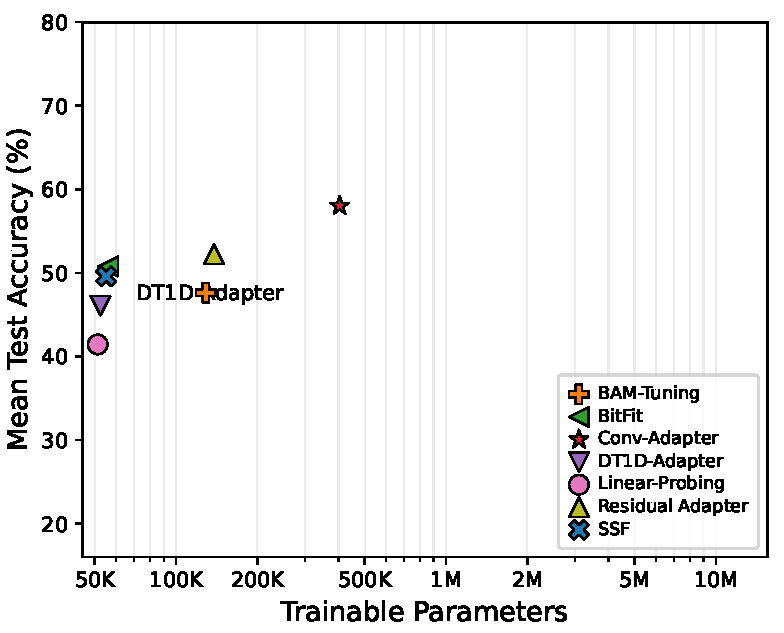
\includegraphics[width=0.94\textwidth]{fig4.pdf}
\caption{Current accuracy--parameter trade-off on FGVC-Aircraft with an ImageNet-pretrained ResNet-18 backbone trained for 10 epochs, using representative seed 0. The figure includes the seven completed F04 methods available in the supplied archive; current Full fine-tuning, LoRA-Conv, and Side-Tuning runs are not available and are therefore not shown.}
\label{fig:fgvc_aircraft_accuracy_params_10ep}
\end{figure*}

\section{Conclusion}
\label{sec:Conclusion}

This paper introduced \textbf{DT1D-Adapter}, a structured parameter-efficient spatial adaptation module for visual backbones. The final formulation represents each group of direct axial kernels using a group-shared symmetric base response on radii $\{1,2,4\}$ and a normalized radius-4 channel-dependent correction. Each axis then learns a bounded $p=2$ symmetric coefficient shift, initialized at zero and fused into an effective 13-tap kernel. The shifted height and width kernels are jointly normalized, executed through one depthwise convolution per axis, and injected through a learned residual gate.

The ablation results support the parameter-compact design. On DTD/ResNet-18, the final method obtains $62.163\pm0.406\%$ test Acc@1 with 25,335 trainable parameters, compared with $61.418\pm0.374\%$ and 89,399 parameters for the unrestricted axial depthwise control. On Flowers102/ResNet-50, the corresponding values are $81.477\pm0.551\%$ with 218,486 parameters versus $80.577\pm0.277\%$ with 722,550 parameters. The learned weighted-shift increment is modest in both settings, whereas removing the post-shift joint $\ell_1$ projection produces the larger accuracy decrease.

The currently complete ViT reruns show that the same spatial interface can be used with Transformer backbones, while also revealing clear limitation cases. On Flowers102 with ViT-B/16, DT1D-Adapter reaches $96.092\pm0.203\%$ test Acc@1 at batch size 32 and $95.864\pm0.191\%$ at batch size 16, using 84,234 trainable parameters. The batch-size-32 result exceeds the supplied Full fine-tuning, VPT, and Linear probing means while remaining below Pfeiffer Adapter ($96.867\pm0.047\%$), which uses 972,966 trainable parameters. On VTAB-Caltech101, DT1D-Adapter reaches $82.249\pm1.078\%$ with 84,234 trainable parameters, closely matching VPT at $82.495\pm1.335\%$ while using slightly fewer trainable parameters. On VTAB-DTD it reaches $49.450\pm1.413\%$ with 41,939 trainable parameters, and on VTAB-EuroSAT it reaches $77.179\pm0.593\%$ with 13,486 trainable parameters. In the latter two settings, stronger raw accuracy is obtained by other supplied baselines. Accordingly, DT1D-Adapter is positioned as a compact structured spatial PEFT alternative rather than a universally dominant method.

The completed PennFudan binary-segmentation reruns provide complementary dense-prediction results. With DeepLabV3-MobileNetV3-Large, DT1D-Adapter obtains $46.345\pm1.288\%$ foreground IoU and $63.330\pm1.197\%$ Dice over three seeds. LoRA-Conv is the strongest supplied PEFT baseline in that experiment at $49.860\pm1.334\%$ IoU, while Full fine-tuning reaches $67.853\pm1.604\%$. DT1D-Adapter nevertheless uses only 792 adapter-specific parameters, compared with 94,208 for LoRA-Conv, 119,364 for Residual Adapters, 212,990 for BAM, and 480,394 for Conv-Adapter. With the ViT-B/16 dense decoder, DT1D-Adapter reaches $64.279\pm0.694\%$ IoU and $78.255\pm0.513\%$ Dice using 1,252 trainable parameters in total, including 483 adapter-specific parameters. BitFit is strongest among the four supplied ViT dense runs at $66.874\pm1.558\%$ IoU, whereas the supplied Full fine-tuning run reaches $39.001\pm0.991\%$. These segmentation results support the compactness of the proposed spatial branch but do not support a claim of universally best raw segmentation accuracy.

The completed D03 semantic-segmentation rerun on Oxford-IIIT Pet provides an additional dense-prediction comparison. Full fine-tuning reaches $77.231\pm0.089\%$ mIoU, while BAM is the strongest supplied PEFT method at $65.475\pm0.590\%$. DT1D-Adapter reaches $63.707\pm0.242\%$ mIoU and $74.105\pm0.250\%$ Dice with only 792 adapter-specific parameters, compared with 212,990 for BAM and 480,394 for Conv-Adapter. Its latency is $3.312\pm0.177$~ms/image, so the D03 result again supports parameter compactness without establishing a universal runtime advantage.

The completed D07 Oxford-IIIT Pet ViT-B/16 semantic-segmentation rerun further tests the same spatial interface with a Transformer backbone. DT1D-Adapter reaches $73.634\pm0.342\%$ mIoU and $83.058\pm0.352\%$ Dice with 2,790 trainable parameters in total, including 483 adapter-specific parameters. BitFit obtains the strongest supplied mean mIoU at $76.671\pm0.246\%$ with 105,219 trainable parameters, while Linear probing reaches $72.635\pm0.035\%$. DT1D-Adapter therefore provides a favorable parameter footprint while remaining below BitFit in raw mIoU under this 5-epoch protocol.

The updated 10-epoch object-detection rerun shows that DT1D-Adapter reaches $96.940\pm0.359\%$ $\mathrm{AP}_{50}$ and $97.911\pm0.713\%$ $\mathrm{Recall}_{50}$ on Oxford-IIIT Pet with Faster R-CNN/MobileNetV3-FPN. BAM obtains the strongest supplied mean $\mathrm{AP}_{50}$ at $98.191\pm0.377\%$, while DT1D-Adapter uses only 792 adapter-specific parameters compared with 212,990 for BAM and 480,394 for Conv-Adapter. The supplied Full fine-tuning detection aggregate remains unstable because two seeds yield zero $\mathrm{AP}_{50}$ and zero $\mathrm{Recall}_{50}$; all supplied runs are retained rather than discarded.

The newly incorporated CNN efficiency profiles reinforce the distinction between parameter efficiency and wall-clock efficiency. On Flowers102/ResNet-18 at 10 epochs, DT1D-Adapter reaches $83.011\pm0.244\%$ test Acc@1 with 53,550 trainable parameters, close to BitFit ($83.157\pm0.474\%$) and SSF ($83.103\pm0.818\%$), while Full fine-tuning reaches $88.415\pm0.206\%$. The corresponding C03 profiler reports 3.686~G FLOPs and $1.770\pm0.117$~ms/image for DT1D-Adapter, versus 1.819~G FLOPs and sub-$0.60$~ms/image latency for the supplied Linear, BitFit, and SSF profiles. On Oxford-IIIT Pet/EfficientNet-B0 at 10 epochs, DT1D-Adapter uses only 48,595 trainable parameters and about 0.185~MiB of FP32 task-specific storage while reaching $91.905\pm0.109\%$ test Acc@1, but its measured $3.995\pm0.466$~ms/image latency is higher than the completed Linear, BitFit, SSF, and Conv-Adapter profiles. On EuroSAT/MobileNetV3-Small, the currently complete C13 Linear-probing row provides a reference profile of $0.758\pm0.010$~ms/image and $1319.887\pm17.330$ FPS. These measurements are therefore reported alongside accuracy and parameter counts rather than treating parameter count as a proxy for runtime efficiency.

Several CNN and other result reruns are still pending in this working manuscript version. In particular, C11 and C13 remain partial beyond the completed rows reported above. Their unavailable table cells remain intentionally blank rather than carrying forward legacy values. The final quantitative discussion should be updated only after the corresponding current reruns are available.
\section*{Acknowledgements}



The authors would like to express their sincere gratitude to the anonymous reviewers and the editor for their valuable comments and constructive suggestions, which significantly improved the quality and clarity of the revised manuscript. The authors also thank their colleagues at Ho Chi Minh City University of Technology (HCMUT) and Hanoi University of Science and Technology (HUST) for their helpful comments and suggestions. In particular, the authors gratefully acknowledge Bao Tran, whose name means ``precious'', of Ho Chi Minh City University of Technology (HCMUT), Vietnam National University Ho Chi Minh City (VNU-HCM), Ho Chi Minh City, Vietnam, for her insightful discussions, thoughtful support, encouragement, and kind care throughout the preparation of this work. 
\section*{Funding}

No funding was received for conducting this study.
\section*{Disclosure statement}

No potential conflict of interest was reported by the author(s).


\section*{Data Availability}

No new dataset was collected or created in this study. The classification
experiments use publicly available benchmarks, including DTD R1.0.1,
Oxford Flowers102, Oxford-IIIT Pet, EuroSAT RGB, Caltech101,
VTAB-Caltech101, VTAB-DTD, and VTAB-EuroSAT. DTD uses official partition~1, Flowers102
uses its official training, validation, and test splits, and the corrected
VTAB-Caltech101, VTAB-DTD, and VTAB-EuroSAT evaluations follow the VTAB-1k protocol~\cite{zhai2019vtab},
using \texttt{train800} for training, \texttt{val200} for validation, and the
official test set for testing. For datasets without a separate
official validation set, the training and validation subsets were generated
from the official training data according to the split protocol described in
the experimental section. The dense-prediction experiments use the publicly
available PennFudan Pedestrian and Oxford-IIIT Pet datasets.

Images were resized to the input resolution reported in the corresponding
tables. Training-time augmentation and deterministic evaluation preprocessing
were applied according to the released experiment configurations, with
ImageNet normalization for ImageNet-pretrained backbones. The accompanying
repository provides the source code, dataset preparation instructions,
configuration files, random seeds, preprocessing settings, experiment
commands, processed logs, and summary result files used to reproduce the
reported tables and figures. \begin{thebibliography}{99}
\bibitem{zhang2026datasetdistillation}
Zhang J, Dai L, Ye F, Chen Z, Li P, Yang X, Sheng B:
Dataset distillation via a noise-unconstrained generative model.
IEEE Trans. Pattern Anal. Mach. Intell., early access (2026).
\href{https://doi.org/10.1109/TPAMI.2026.3690778}
{doi: 10.1109/TPAMI.2026.3690778}

\bibitem{lin2023eapt}
Lin X, Sun S, Huang W, Sheng B, Li P, Feng DD:
EAPT: Efficient attention pyramid transformer for image processing.
IEEE Trans. Multimedia 25, 50--61 (2023).
Published online 20 October 2021.
\href{https://doi.org/10.1109/TMM.2021.3120873}
{doi: 10.1109/TMM.2021.3120873}

\bibitem{wen2025retinalvessel}
Wen Y, Shen S, Shi W, Cao W, Bi L, Yang X, Sheng B:
A lightweight depthwise separable ConvNet with frequency-domain enhancement
for retinal vessel segmentation.
ACM Trans. Multimedia Comput. Commun. Appl. 21(12),
Article 336, 1--23 (2025).
\href{https://doi.org/10.1145/3767732}
{doi: 10.1145/3767732}

\bibitem{wang2025anisym}
Wang J, Lu X, Bennamoun M, Sheng B:
Non-rigid point cloud registration via anisotropic hybrid field harmonization.
IEEE Trans. Pattern Anal. Mach. Intell. 47(9), 7898--7915 (2025).
\href{https://doi.org/10.1109/TPAMI.2025.3572584}
{doi: 10.1109/TPAMI.2025.3572584}

\bibitem{wu2025eyefm}
Wu Y, Qian B, Li T, et al:
An eyecare foundation model for clinical assistance:
A randomized controlled trial.
Nat. Med. 31(10), 3404--3413 (2025).
\href{https://doi.org/10.1038/s41591-025-03900-7}
{doi: 10.1038/s41591-025-03900-7}

\bibitem{meng2025deepdkd}
Meng Z, Guan Z, Yu S, et al:
Non-invasive biopsy diagnosis of diabetic kidney disease via deep learning
applied to retinal images: A population-based study.
Lancet Digit. Health 7(5), Article 100868 (2025).
\href{https://doi.org/10.1016/j.landig.2025.02.008}
{doi: 10.1016/j.landig.2025.02.008}
\bibitem{wang2007pennfudan}
Wang L, et al:
Object detection combining recognition and segmentation.
In: Proc. ACCV, LNCS, vol. 4843, pp. 189--199 (2007).
\href{https://doi.org/10.1007/978-3-540-76386-4_17}{doi: 10.1007/978-3-540-76386-4\_17}


\bibitem{howard2019mobilenetv3}
Howard A, et al:
Searching for MobileNetV3.
In: Proc. ICCV, pp. 1314--1324 (2019).
\href{https://doi.org/10.1109/ICCV.2019.00140}{doi: 10.1109/ICCV.2019.00140}

\bibitem{huang2017densenet}
Huang G, Liu Z, van der Maaten L, Weinberger KQ:
Densely connected convolutional networks.
In: Proc. CVPR, pp. 4700--4708 (2017).
\href{https://doi.org/10.1109/CVPR.2017.243}{doi: 10.1109/CVPR.2017.243}

\bibitem{he2016resnet}
He K, et al:
Deep residual learning for image recognition.
In: Proc. CVPR, pp. 770--778 (2016).
\href{https://doi.org/10.1109/CVPR.2016.90}{doi: 10.1109/CVPR.2016.90}

\bibitem{dosovitskiy2021vit}
Dosovitskiy A, et al:
An image is worth $16\times16$ words: Transformers for image recognition at scale.
In: Proc. ICLR (2021)

\bibitem{houlsby2019adapter}
Houlsby N, et al:
Parameter-efficient transfer learning for NLP.
In: Proc. ICML, PMLR, vol. 97, pp. 2790--2799 (2019).

\bibitem{hu2022lora}
Hu EJ, et al:
LoRA: Low-rank adaptation of large language models.
In: Proc. ICLR (2022)

\bibitem{zaken2022bitfit}
Ben Zaken E, et al:
BitFit: Simple parameter-efficient fine-tuning for transformer-based masked language models.
In: Proc. ACL, Short Papers, pp. 1--9 (2022).
\href{https://doi.org/10.18653/v1/2022.acl-short.1}{doi: 10.18653/v1/2022.acl-short.1}

\bibitem{jia2022vpt}
Jia M, et al:
Visual prompt tuning.
In: Proc. ECCV, pp. 709--727 (2022).
\href{https://doi.org/10.1007/978-3-031-19827-4_41}{doi: 10.1007/978-3-031-19827-4\_41}

\bibitem{lian2022ssf}
Lian D, et al:
Scaling \& shifting your features: A new baseline for efficient model tuning.
In: Adv. Neural Inf. Process. Syst., vol. 35, pp. 109--123 (2022).
\href{https://doi.org/10.52202/068431-0009}{doi: 10.52202/068431-0009}

\bibitem{chen2022adaptformer}
Chen S, et al:
AdaptFormer: Adapting vision transformers for scalable visual recognition.
In: Adv. Neural Inf. Process. Syst., vol. 35, pp. 16664--16678 (2022).
\href{https://doi.org/10.52202/068431-1212}{doi: 10.52202/068431-1212}

\bibitem{jie2024convpass}
Jie S, et al:
Convolutional bypasses are better vision transformer adapters.
In: Proc. ECAI, Front. Artif. Intell. Appl., vol. 392, pp. 202--209 (2024).
\href{https://doi.org/10.3233/FAIA240489}{doi: 10.3233/FAIA240489}

\bibitem{luo2023repadapter}
Luo G, et al:
Towards efficient visual adaption via structural re-parameterization.
arXiv preprint arXiv:2302.08106 (2023).
\href{https://doi.org/10.48550/arXiv.2302.08106}{doi: 10.48550/arXiv.2302.08106}

\bibitem{li2024repadapter}
Li C, et al:
Rep-Adapter: Parameter-free automatic adaptation of pre-trained ConvNets via re-parameterization.
In: Proc. ICLR (2024)

\bibitem{cai2020tinytl}
Cai H, et al:
TinyTL: Reduce memory, not parameters for efficient on-device learning.
In: Adv. Neural Inf. Process. Syst., vol. 33, pp. 11285--11297 (2020)

\bibitem{he2023spt}
He H, et al:
Sensitivity-aware visual parameter-efficient fine-tuning.
In: Proc. ICCV, pp. 11791--11801 (2023).
\href{https://doi.org/10.1109/ICCV51070.2023.01086}{doi: 10.1109/ICCV51070.2023.01086}

\bibitem{yu2022vpetl}
Yu BXB, et al:
Towards a unified view on visual parameter-efficient transfer learning.
arXiv preprint arXiv:2210.00788 (2022).
\href{https://doi.org/10.48550/arXiv.2210.00788}{doi: 10.48550/arXiv.2210.00788}

\bibitem{mai2025unifying}
Mai Z, et al:
Lessons and insights from a unifying study of parameter-efficient fine-tuning (PEFT) in visual recognition.
In: Proc. CVPR, pp. 14845--14857 (2025).
\href{https://doi.org/10.1109/CVPR52734.2025.01383}{doi: 10.1109/CVPR52734.2025.01383}

\bibitem{xin2024vpetlbench}
Xin Y, et al:
V-PETL Bench: A unified visual parameter-efficient transfer learning benchmark.
In: Adv. Neural Inf. Process. Syst., vol. 37, pp. 80522--80535,
Datasets and Benchmarks Track (2024).
\href{https://doi.org/10.52202/079017-2560}{doi: 10.52202/079017-2560}

\bibitem{yu2024visualtuning}
Yu BXB, et al:
Visual tuning.
ACM Comput. Surv. 56(12), Article 297, 1--38 (2024).
\href{https://doi.org/10.1145/3657632}{doi: 10.1145/3657632}

\bibitem{xin2024visionpeftsurvey}
Xin Y, et al:
Parameter-efficient fine-tuning for pre-trained vision models: A survey and benchmark.
Int. J. Comput. Vis. 134(6), Article 304 (2026).
\href{https://doi.org/10.1007/s11263-026-02864-6}{doi: 10.1007/s11263-026-02864-6}

\bibitem{howard2017mobilenet}
Howard AG, et al:
MobileNets: Efficient convolutional neural networks for mobile vision applications.
arXiv preprint arXiv:1704.04861 (2017).
\href{https://doi.org/10.48550/arXiv.1704.04861}{doi: 10.48550/arXiv.1704.04861}

\bibitem{yu2016dilated}
Yu F, Koltun V:
Multi-scale context aggregation by dilated convolutions.
In: Proc. ICLR (2016)

\bibitem{xie2017resnext}
Xie S, et al:
Aggregated residual transformations for deep neural networks.
In: Proc. CVPR, pp. 5987--5995 (2017).
\href{https://doi.org/10.1109/CVPR.2017.634}{doi: 10.1109/CVPR.2017.634}

\bibitem{touvron2021layerscale}
Touvron H, et al:
Going deeper with image transformers.
In: Proc. ICCV, pp. 32--42 (2021).
\href{https://doi.org/10.1109/ICCV48922.2021.00010}{doi: 10.1109/ICCV48922.2021.00010}

\bibitem{nilsback2008flowers}
Nilsback ME, Zisserman A:
Automated flower classification over a large number of classes.
In: Proc. ICVGIP, pp. 722--729 (2008).
\href{https://doi.org/10.1109/ICVGIP.2008.47}{doi: 10.1109/ICVGIP.2008.47}

\bibitem{netzer2011svhn}
Netzer Y, et al:
Reading digits in natural images with unsupervised feature learning.
In: NIPS Workshop on Deep Learning and Unsupervised Feature Learning (2011)

\bibitem{parkhi2012pets}
Parkhi OM, et al:
Cats and dogs.
In: Proc. CVPR, pp. 3498--3505 (2012).
\href{https://doi.org/10.1109/CVPR.2012.6248092}{doi: 10.1109/CVPR.2012.6248092}

\bibitem{bossard2014food101}
Bossard L, et al:
Food-101 -- Mining discriminative components with random forests.
In: Proc. ECCV, pp. 446--461 (2014).
\href{https://doi.org/10.1007/978-3-319-10599-4_29}{doi: 10.1007/978-3-319-10599-4\_29}

\bibitem{chen2024convadapter}
Chen H, et al:
Conv-Adapter: Exploring parameter efficient transfer learning for ConvNets.
In: Proc. CVPRW, pp. 1551--1561 (2024).
\href{https://doi.org/10.1109/CVPRW63382.2024.00162}{doi: 10.1109/CVPRW63382.2024.00162}

\bibitem{maji2013fgvcaircraft}
Maji S, et al:
Fine-grained visual classification of aircraft.
arXiv preprint arXiv:1306.5151 (2013).
\href{https://doi.org/10.48550/arXiv.1306.5151}{doi: 10.48550/arXiv.1306.5151}


\bibitem{rebuffi2017residual}
Rebuffi SA, et al:
Learning multiple visual domains with residual adapters.
In: Adv. Neural Inf. Process. Syst., vol. 30 (2017)

\bibitem{zhang2025pdft}
Zhang M, et al:
PDFT: Parameter-diminish fine-tuning for transformer-based models.
Vis. Comput. 41(9), 6745--6755 (2025).
\href{https://doi.org/10.1007/s00371-025-03973-y}{doi: 10.1007/s00371-025-03973-y}

\bibitem{zhang2025lightweightcnnvit}
Zhang G, et al:
Lightweight CNN--ViT with cross-module representational constraint for express parcel detection.
Vis. Comput. 41(5), 3283--3295 (2025).
\href{https://doi.org/10.1007/s00371-024-03602-0}{doi: 10.1007/s00371-024-03602-0}

\bibitem{zhu2024ceal}
Zhu J, et al:
Clustering environment aware learning for active domain adaptation.
IEEE Trans. Syst. Man Cybern. Syst. 54(6), 3891--3904 (2024).
\href{https://doi.org/10.1109/TSMC.2024.3374068}{doi: 10.1109/TSMC.2024.3374068}

\bibitem{park2020lightweightattention}
Park J, et al:
A simple and light-weight attention module for convolutional neural networks.
Int. J. Comput. Vis. 128(4), 783--798 (2020).
\href{https://doi.org/10.1007/s11263-019-01283-0}{doi: 10.1007/s11263-019-01283-0}

\bibitem{chollet2017xception}
Chollet F:
Xception: Deep learning with depthwise separable convolutions.
In: Proc. CVPR, pp. 1800--1807 (2017).
\href{https://doi.org/10.1109/CVPR.2017.195}{doi: 10.1109/CVPR.2017.195}

\bibitem{hu2020senet}
Hu J, et al:
Squeeze-and-excitation networks.
IEEE Trans. Pattern Anal. Mach. Intell. 42(8), 2011--2023 (2020).
\href{https://doi.org/10.1109/TPAMI.2019.2913372}{doi: 10.1109/TPAMI.2019.2913372}

\bibitem{hedegaard2024spa}
Hedegaard L, et al:
Structured pruning adapters.
Pattern Recognit. 156, Article 110724 (2024).
\href{https://doi.org/10.1016/j.patcog.2024.110724}{doi: 10.1016/j.patcog.2024.110724}

\bibitem{xu2024lvadapter}
Xu G, et al:
Lv-Adapter: Adapting Vision Transformers for visual classification with linear-layers and vectors.
Comput. Vis. Image Underst. 246, Article 104049 (2024).
\href{https://doi.org/10.1016/j.cviu.2024.104049}{doi: 10.1016/j.cviu.2024.104049}

\bibitem{gao2024clipadapter}
Gao P, et al:
CLIP-Adapter: Better vision--language models with feature adapters.
Int. J. Comput. Vis. 132(2), 581--595 (2024).
\href{https://doi.org/10.1007/s11263-023-01891-x}{doi: 10.1007/s11263-023-01891-x}

\bibitem{park2026peftmetar}
Park J, et al:
Parameter-efficient fine-tuning via meta-regularizer.
Int. J. Comput. Vis. 134, Article 148 (2026).
\href{https://doi.org/10.1007/s11263-025-02693-z}{doi: 10.1007/s11263-025-02693-z}

\bibitem{ho2019axialattention}
Ho J, et al:
Axial attention in multidimensional transformers.
arXiv preprint arXiv:1912.12180 (2019).
\href{https://doi.org/10.48550/arXiv.1912.12180}{doi: 10.48550/arXiv.1912.12180}

\bibitem{wang2020axialdeeplab}
Wang H, et al:
Axial-DeepLab: Stand-alone axial-attention for panoptic segmentation.
In: Proc. ECCV, pp. 108--126 (2020).
\href{https://doi.org/10.1007/978-3-030-58548-8_7}{doi: 10.1007/978-3-030-58548-8\_7}

\bibitem{hou2021coordinateattention}
Hou Q, et al:
Coordinate attention for efficient mobile network design.
In: Proc. CVPR, pp. 13708--13717 (2021).
\href{https://doi.org/10.1109/CVPR46437.2021.01350}{doi: 10.1109/CVPR46437.2021.01350}

\bibitem{luo2016effectiveRF}
Luo W, et al:
Understanding the effective receptive field in deep convolutional neural networks.
In: Adv. Neural Inf. Process. Syst., vol. 29 (2016)

\bibitem{liu2022convnext}
Liu Z, et al:
A ConvNet for the 2020s.
In: Proc. CVPR, pp. 11966--11976 (2022).
\href{https://doi.org/10.1109/CVPR52688.2022.01167}{doi: 10.1109/CVPR52688.2022.01167}

\bibitem{ding2022replknet}
Ding X, et al:
Scaling up your kernels to $31\times31$: Revisiting large kernel design in CNNs.
In: Proc. CVPR, pp. 11953--11965 (2022).
\href{https://doi.org/10.1109/CVPR52688.2022.01166}{doi: 10.1109/CVPR52688.2022.01166}

\bibitem{zhang2025noah}
Zhang Y, et al:
Neural prompt search.
IEEE Trans. Pattern Anal. Mach. Intell. 47(7), 5268--5280 (2025).
\href{https://doi.org/10.1109/TPAMI.2024.3435939}{doi: 10.1109/TPAMI.2024.3435939}

\bibitem{jie2023fact}
Jie S, Deng ZH:
FacT: Factor-Tuning for lightweight adaptation on Vision Transformer.
Proc. AAAI Conf. Artif. Intell. 37(1), 1060--1068 (2023).
\href{https://doi.org/10.1609/aaai.v37i1.25187}{doi: 10.1609/aaai.v37i1.25187}

\bibitem{chen2023vitadapter}
Chen Z, et al:
Vision Transformer Adapter for dense predictions.
In: Proc. ICLR (2023)

\bibitem{yin2023lorand}
Yin D, et al:
$1\%$ VS $100\%$: Parameter-efficient low rank adapter for dense predictions.
In: Proc. CVPR, pp. 20116--20126 (2023).
\href{https://doi.org/10.1109/CVPR52729.2023.01926}{doi: 10.1109/CVPR52729.2023.01926}

\bibitem{yin2025mona}
Yin D, et al:
$5\%>100\%$: Breaking performance shackles of full fine-tuning on visual recognition tasks.
In: Proc. CVPR, pp. 20071--20081 (2025).
\href{https://doi.org/10.1109/CVPR52734.2025.01869}{doi: 10.1109/CVPR52734.2025.01869}

\bibitem{chen2018deeplab}
Chen LC, et al:
DeepLab: Semantic image segmentation with deep convolutional nets, atrous convolution, and fully connected CRFs.
IEEE Trans. Pattern Anal. Mach. Intell. 40(4), 834--848 (2018).
\href{https://doi.org/10.1109/TPAMI.2017.2699184}{doi: 10.1109/TPAMI.2017.2699184}

\bibitem{li2019sknet}
Li X, et al:
Selective kernel networks.
In: Proc. CVPR, pp. 510--519 (2019).
\href{https://doi.org/10.1109/CVPR.2019.00060}{doi: 10.1109/CVPR.2019.00060}

\bibitem{grafakos2014classical}
Grafakos L:
Classical Fourier Analysis.
3rd edn. Grad. Texts Math., vol. 249.
Springer, New York (2014).
\href{https://doi.org/10.1007/978-1-4939-1194-3}{doi: 10.1007/978-1-4939-1194-3}

\bibitem{mallat2009wavelet}
Mallat S:
A Wavelet Tour of Signal Processing: The Sparse Way.
3rd edn. Academic Press, Burlington (2009).
\href{https://doi.org/10.1016/B978-0-12-374370-1.X0001-8}{doi: 10.1016/B978-0-12-374370-1.X0001-8}

\bibitem{fei2007caltech101}
Fei-Fei L, et al:
Learning generative visual models from few training examples: An incremental Bayesian approach tested on 101 object categories.
Comput. Vis. Image Underst. 106(1), 59--70 (2007).
\href{https://doi.org/10.1016/j.cviu.2005.09.012}{doi: 10.1016/j.cviu.2005.09.012}


\bibitem{jaccard1912distribution}
Jaccard P:
The distribution of the flora in the Alpine zone.
New Phytol. 11(2), 37--50 (1912).
\href{https://doi.org/10.1111/j.1469-8137.1912.tb05611.x}{doi: 10.1111/j.1469-8137.1912.tb05611.x}

\bibitem{dice1945measures}
Dice LR:
Measures of the amount of ecologic association between species.
Ecology 26(3), 297--302 (1945).
\href{https://doi.org/10.2307/1932409}{doi: 10.2307/1932409}

\bibitem{everingham2010pascal}
Everingham M, et al:
The PASCAL Visual Object Classes (VOC) challenge.
Int. J. Comput. Vis. 88(2), 303--338 (2010).
\href{https://doi.org/10.1007/s11263-009-0275-4}{doi: 10.1007/s11263-009-0275-4}

\bibitem{lin2014coco}
Lin TY, et al:
Microsoft COCO: Common objects in context.
In: Proc. ECCV, pp. 740--755 (2014).
\href{https://doi.org/10.1007/978-3-319-10602-1_48}{doi: 10.1007/978-3-319-10602-1\_48}

\bibitem{zhang2020sidetuning}
Zhang JO, et al:
Side-Tuning: A baseline for network adaptation via additive side networks.
In: Proc. ECCV, LNCS, vol. 12348, pp. 698--714 (2020).
\href{https://doi.org/10.1007/978-3-030-58580-8_41}{doi: 10.1007/978-3-030-58580-8\_41}

\bibitem{shao2025hlora}
Shao Z, et al:
High-level LoRA and hierarchical fusion for enhanced micro-expression recognition.
Vis. Comput. 41(7), 4533--4546 (2025).
\href{https://doi.org/10.1007/s00371-024-03676-w}{doi: 10.1007/s00371-024-03676-w}

\bibitem{lu2026frozenrgbir}
Lu B, et al:
Enhancing RGB-IR object detection: A frozen backbone approach with multi-receptive field attention.
Vis. Comput. 42(3), Article 164 (2026).
\href{https://doi.org/10.1007/s00371-026-04378-1}{doi: 10.1007/s00371-026-04378-1}


\bibitem{zhai2019vtab}
Zhai X, et al:
A large-scale study of representation learning with the Visual Task Adaptation Benchmark.
arXiv preprint arXiv:1910.04867 (2019).
\href{https://doi.org/10.48550/arXiv.1910.04867}{doi: 10.48550/arXiv.1910.04867}

\bibitem{HuongTy2026Applications}
Huong TK, Ty DB:
Application of the $h$-Hartley--cosine convolution on $\mathbb{T}_h$ to integral equations and signal analysis.
Differ. Equ. Dyn. Syst., published online 16 July 2026.
\href{https://doi.org/10.1007/s12591-026-00780-2}
{doi: 10.1007/s12591-026-00780-2}


\bibitem{coates2011stl10}
Coates A, Ng A, Lee H:
An analysis of single-layer networks in unsupervised feature learning.
In: Proc. Fourteenth Int. Conf. Artificial Intelligence and Statistics (AISTATS), PMLR 15, pp. 215--223 (2011).

\bibitem{nilsback2006flowers17}
Nilsback M-E, Zisserman A:
A visual vocabulary for flower classification.
In: Proc. IEEE Conf. Computer Vision and Pattern Recognition (CVPR), vol. 2, pp. 1447--1454 (2006).

\end{thebibliography}
\end{document}
 